\documentclass[12pt]{article}
\usepackage[english]{babel}
\usepackage{fullpage, enumitem, amsmath, amssymb, graphicx, chemformula, stmaryrd, physics, booktabs, float, xfrac, mdframed, blindtext, fancyhdr, pythontex, makecell, pgfplotstable, caption}
\usepackage[left=20mm,right=20mm,top=15mm,bottom=15mm,includeheadfoot]{geometry}

\DeclareMathSymbol{*}{\mathbin}{symbols}{"01}

\usepackage{siunitx}
\sisetup{round-mode=places, round-precision=3}
\newcommand{\pow}[1]{\tothe{#1}}

\usepackage{pgfplots}
\pgfplotsset{compat=1.17}
\usepgfplotslibrary{groupplots}
\usetikzlibrary{matrix,calc}


\usepackage[notextcomp]{kpfonts}

\newcounter{question}[question]
\setcounter{question}{1}

\mdfdefinestyle{question}{
backgroundcolor=black!10, roundcorner=8pt, hidealllines=true, nobreak
}

\def\checkmark{\tikz\fill[scale=0.4](0,.35) -- (.25,0) -- (1,.7) -- (.25,.15) -- cycle;} 

\fancypagestyle{plain}{
\fancyhf{}%
\fancyhead[R]{}
\fancyhead[L]{}
\fancyhead[C]{}
\fancyfoot[R]{\thepage} 
\fancyfoot[C]{}
\fancyfoot[L]{Chemical Reaction Engineering}
\renewcommand{\footrulewidth}{0.4pt}
\renewcommand{\headrulewidth}{0pt}
}

\newenvironment{question}
    {\textbf{Question\;\thequestion}
    \begin{mdframed}[style=question]}
        %% Question Text %%   
    {\end{mdframed}
    \addtocounter{question}{1}} 
    
\newenvironment{solution}
    {}
        %% Solution Text %%   
    {\setcounter{equation}{0}
     \setcounter{table}{0}
    \newpage} 
   
    
\title{Chemical Reaction Engineering - Exam Questions}
\author{Fabian Hofmann -- \texttt{fabian.hofmann@jku.at}}

\setlength{\parindent}{0pt}
\definecolor{myblue}{cmyk}{1,.72,0,.38}

\makeatletter
\renewcommand{\section}{\@startsection{section}{1}{0mm}%
                                {1ex}%
                                {0.5ex}%x
                                {\color{myblue}\Large\bfseries}}
\renewcommand{\subsection}{\@startsection{subsection}{1}{0mm}%
                                {0.5ex}%
                                {0.5ex}%x
                                {\large\bfseries}}
\renewcommand{\subsubsection}{\@startsection{subsubsection}{1}{0mm}%
                                {0.5ex}%
                                {0.5ex}%x
                                {\bfseries}}
\makeatother

\begin{document}

\newcommand{\pySI}[2]{\py{'\\SI{' + str(#1) + '}{#2}'}}
\newcommand{\pyNum}[1]{\py{'\\num{' + str(#1) + '}'}}
\newcommand{\pySIsci}[2]{\py{'\\SI[scientific-notation=true]{' + str(#1) + '}{#2}'}}


\pagestyle{plain}
\maketitle

\begin{question}
In an indirectly cooled CSTR with a heat exchange surface of $F_W = \SI{7}{\square\meter}$, a strongly exothermic irreversible 1st order rection takes place. Initial investigations showed that the heat exchange surface must be increased by installing cooling coils inside the reactor so that the amount of heat produced can be sufficiently dissipated. The reactant is to be fed into the CSTR at a concentration of \SI{1600}{\mole\per\cubic\meter} with a volume flow of \SI{2.3}{\cubic\meter\per\hour}. The temperature of the feed mixture shall be $T_a = \SI{70}{\celsius}$. In the steady state, the operating temperature should be \SI{118}{\celsius}. The average coolant temperature $T_K$ should be \SI{95}{\celsius}. With the selected reaction conditions and operating parameters, a conversion of the reactant of \SI{98}{\percent} can be achieved. 

Further material data: Heat transfer coefficient $k_W = \SI{4. 75e5}{\joule\per\square\meter\per\hour\per\kelvin}$, reaction enthalpy $\Delta H = \SI{-195}{\kilo\joule\per\mole}$, mean density $\rho = \SI{1800}{\kilo\gram\per\cubic\meter}$ and mean specific heat capacity $c_p = \SI{2200}{\joule\per\kelvin\per\kilo\gram}$.
%
\renewcommand{\labelenumi}{\alph{enumi})}
\begin{enumerate}
\item Determine the area that must be provided for additional heat dissipation by installing cooling coils. Establish the heat balance of the statinary CSTR. What is the total area for heat exchange.
\item Give the relative cooling intensity (Stanton number) for the steady state. Also calculate the adiabatic temperature increase.
\end{enumerate}
\end{question}
%%%%%%%%%%%%%%%%%%%%%%%%%%%% Start Python calculations %%%%%%%%%%%%%%%%%%%%%%%%%%%%
\begin{pycode}
import numpy as np
import sympy as sp

# Given data
Fw = 7 #m^2
cA0 = 1600 #mol/m^3
Vdot = 2.3 #m^3/h
Ta = 70 #°C
T = 118 #°C
Tk = 95 #°C
X = 0.98 #%
kW = 4.75e5 #J/(m^2 h K)
DeltaH = -195 #kJ/mol
rho = 1809 #kg/m^3
cp = 2200 #J/(K kg)

#Calculation of the adibatic temperature increase
DeltaTad = (-1000 * DeltaH * cA0)/(rho * cp)

#Calculation of the Stanton number
St = (Ta - T + DeltaTad * X)/(T - Tk)

#Calculation of the needed heat exchange surface
FwNeed = (St * Vdot * rho * cp)/kW

#Calculation of the heat exchange surface which has to be added
FwAdd = FwNeed - Fw

\end{pycode}
%%%%%%%%%%%%%%%%%%%%%%%%%%%% End Python calculations %%%%%%%%%%%%%%%%%%%%%%%%%%%%
\begin{solution}
The heat balance of the CSTR:
%
\begin{equation}\label{eqn1:HB}
T - T_a + St*(T - T_k) = \Delta T_{ad} * X
\end{equation}
%
The adiabatic temperature increase can be calculated by:
%
\begin{equation}
\Delta T_{ad} = \frac{-\Delta H * c_{A0}}{-\nu_A * \rho * c_p} = \pySI{DeltaTad}{\kelvin} 
\end{equation}
%
By rearranging Eq. \ref{eqn1:HB} the Stanton number can be calculated
%
\begin{equation}
St = \frac{T_a - T + \Delta T_{ad} * X}{T - T_k} = \pyNum{St}
\end{equation}
%
The heat exchange surface still to be installed can be calculated according to:
%
\begin{equation}
F_{W,add} = \frac{St * \dot{V} * \rho * c_p}{k_W} - F_W = \pySI{FwAdd}{\square\meter}
\end{equation}
\end{solution}
\begin{question}
During the execution of a radical polymerization at \SI{125}{\celsius} with an initial initiator concentration of $c_{I0} = \SI{0.001}{\mol\per\liter}$, the following kinetic data were determined: The rate constant of the initiator decomposition reaction $k_z = \SI{1.09e-11}{\per\second}$, the gross rate constant $k_{Br} = \SI{3.09e-3}{\liter\tothe{1\per 2}\per\mole\tothe{1\per 2}\per\second}$
%
\renewcommand{\labelenumi}{\alph{enumi})}
\begin{enumerate}
\item Calculate the polymerisation time until a monomer conversion of \SI{70}{\percent} is reached. Write down the formulae you used for this calculation.
\end{enumerate}
\end{question}
%%%%%%%%%%%%%%%%%%%%%%%%%%%% Start Python calculations %%%%%%%%%%%%%%%%%%%%%%%%%%%%
\begin{pycode}
import numpy as np
import sympy as sp

t = sp.symbols('t', positive=True, real=True)

# Given data
T = 125 + 273.15 #K
cI0 = 0.001 #mol/L
kz = 1.09e-11 #s^-1
kBr = 3.09e-3 #L^0.5 mol^-0.5 s^-1
X = 0.7

# Calculation of the polymerization time
sol = sp.solve((2 * kBr * sp.sqrt(cI0)) / kz * (sp.exp(-kz * t / 2) - 1) - sp.log(1 - X), t)
\end{pycode}
%%%%%%%%%%%%%%%%%%%%%%%%%%%% End Python calculations %%%%%%%%%%%%%%%%%%%%%%%%%%%%
\begin{solution}
The logarithmic ratio of the monomer concentration to the initial concentration can be calculated by (CRE exercise 6):
%
\begin{equation}\label{eqn2:ratio}
\ln \left( \frac{c_M}{c_{M0}} \right) = \frac{2 * k_{Br} * \sqrt{c_{I0}}}{k_z} * \left[ \exp\left(\frac{-k_z * t}{2} \right) - 1 \right]
\end{equation}
%
The conversion in constant reaction volume is defined by:
%
\begin{equation}
X = \frac{c_{M0} - c_M}{c_{M0}} \Longrightarrow \frac{c_M}{c_{M0}} = 1 - X
\end{equation}
%
Thus Eq. \ref{eqn2:ratio} can be rearranged to:
%
\begin{align}
\begin{split}
&\ln \left( 1 - X \right) = \frac{2 * k_{Br} * \sqrt{c_{I0}}}{k_z} * \left[ \exp\left(\frac{-k_z * t}{2} \right) - 1 \right]\\
&\Longrightarrow t = -\frac{2}{k_z} * \ln \left[ \frac{\ln (1 - X) * k_z}{2 * k_{Br} * \sqrt{c_{I0}}} + 1 \right] = \pySI{sol[0]}{\second}
\end{split} 
\end{align}
\end{solution}

\begin{question}
Butyl acetat shall be produced at \SI{100}{\celsius} from acetic acid and butanol with suphuric acid as catalyst.
%%
\begin{equation*}
\ch{CH3COOH + C4H9OH -> CH3COOC4H9 + H2O}
\end{equation*}
%%
After a first approximation, it is a 2nd order reaction: \\
$r = k * c_A * c_B$ with $k = \SI{0.03}{\liter\per\mole\per\minute}$. The reaction should be terminated at a conversion of $X_A = 0.69$. The component react only in the desired form to form the butyl ester, so that the selectivity can be set to one. The production rate of the butyl ester should be \SI{109}{\kilo\gram\per\hour}. The dead time of the batch reactor for filling, heating, cooling and emptying is \SI{15}{\minute} (additional to the reaction time). The initial concentration of acetic acid is $c_{A0} = \SI{2}{\mole\per\liter}$ 
\renewcommand{\labelenumi}{\alph{enumi})}
\begin{enumerate}
 \item Calculate the Damköhler number.
 \item Calculate the residence time $\tau$.
 \item Calculate the reaction volume $V_R$ of the batch reactor.
\end{enumerate}
\end{question}
%%%%%%%%%%%%%%%%%%%%%%%%%%%% Start Python calculations %%%%%%%%%%%%%%%%%%%%%%%%%%%%
\begin{pycode}
# Given data
Mp = 116 #g mol^-1
Xa = 0.69
Sp = 1
mDot = 109 #kg h^-1
k = 0.03 #L mol^-1 min^-1
cA0 = 2 #mol/L
tD = 15 #min

# Calculation of the Damkoehler number
Da = Xa/(1-Xa)

# Calculation of the residence time
tau = Da/(k * cA0)

# Calculation of the reaction volume
Vr = 1000/60 * mDot/Mp * (tau + tD)/(cA0*Sp*Xa)
\end{pycode}
%%%%%%%%%%%%%%%%%%%%%%%%%%%% End Python calculations %%%%%%%%%%%%%%%%%%%%%%%%%%%%
\begin{solution}
The Damköhler number for a batch reactor and a reaction of 2nd order can be calculated by:
%
\begin{align}
\begin{split}
Da &= \int\limits_0^{X_A} \frac{1}{\Phi(X)}\;\mathrm{d}X = \int\limits_0^{X_A} \frac{1}{(1 - X)^2}\;\mathrm{d}X \\
&= \frac{X_A}{1 - X_A} = \pyNum{Da}
\end{split}
\end{align}
%%
The residence time can be calculated by:
%%
\begin{equation}
\tau = \frac{Da * c_{A0}}{-\nu_A * r_0} = \frac{Da}{-\nu_A * k * c_{A0}} = \pySI{tau}{\minute}
\end{equation}
%%
The selectivity towards the product can be calculated by:
%%
\begin{equation}
S_P = \frac{n_P - n_{P0}}{n_{A0} - n_A} * \frac{-\nu_A}{\nu_P} \Longrightarrow n_{A0} - n_A = \frac{n_P - n_{P0}}{S_P} * \frac{-\nu_A}{\nu_P}
\end{equation}
%%
The conversion of educt A is defined by:
%%
\begin{align}
\begin{split}
&X_A = \frac{n_{A0} - n_A}{n_{A0}} = \frac{n_P - n_{P0}}{n_{A0} * S_P} * \frac{-\nu_A}{\nu_P}\\
&\Longrightarrow n_P - n_{P0} = \frac{\nu_P}{-\nu_A} * n_{A0} * S_P * X_A
\end{split}
\end{align}
%%
The production rate is defined by:
%%
\begin{equation}\label{eqn3:dotn}
\dot{n}_P = \frac{\dot{m}_P}{M_P} = \frac{n_P - n_{P0}}{\tau + t_d} = \frac{\nu_P}{-\nu_A} * n_{A0} * S_P * X_A * \frac{1}{\tau + t_d}
\end{equation}
%%
With $n_{A0} = c_{A0} * V_R$ the reactor volume $V_R$ can be calculated by rearranging Eq. \ref{eqn3:dotn}:
%%
\begin{equation}
V_R = \frac{\dot{m}_P}{M_P} * \frac{-\nu_A}{\nu_P} * \frac{\tau + t_d}{c_{A0} * S_P * X_A} =  \pySI{Vr}{\liter}
\end{equation}
\end{solution}

\begin{question}
For a zero order reaction, the following applies: $X = Da$
%%
\renewcommand{\labelenumi}{\alph{enumi})}
\begin{enumerate}
 \item What conversion do you expect with $Da = 2$
 \item Is the Damköhler number at this reaction order depended on the temperature?
 \item How do you explain this? Use equations for the explanation!
\end{enumerate}
\end{question}
%%%%%%%%%%%%%%%%%%%%%%%%%%%% Start Python calculations %%%%%%%%%%%%%%%%%%%%%%%%%%%%
\begin{pycode}

\end{pycode}
%%%%%%%%%%%%%%%%%%%%%%%%%%%% End Python calculations %%%%%%%%%%%%%%%%%%%%%%%%%%%%
\begin{solution}
The conversion can only be \SI{100}{\percent} even if $Da = 2$. The higher Damköhler number can be attributed to the temperature.
%%
\begin{equation}
Da = \frac{-\nu_A * r_0 * \tau}{c_{A0}}
\end{equation}
The reaction rate $r_0$ at the begin of the reaction $(X = 0)$:
%%
\begin{equation}
r_0 = k(T) = k_{\infty} * \exp\left(\frac{-E_A}{R * T}\right)
\end{equation}
\end{solution}

\begin{question}
For an exothermic reaction, draw the expected course of reaction of the educt A $(c_A)$ as a functiuon of time $(t)$ and location $(x)$ espacially for the measurement location $z_0$ and $z_1$. The reaction proceeds according to the scheme
%%
\begin{equation*}
\ch{A -> P}
\end{equation*}
No cooling and the reactors behave ideal.
\end{question}
\begin{solution}
Time and location dependence on concentration:
\begin{center}
% This file was created by tikzplotlib v0.9.8.
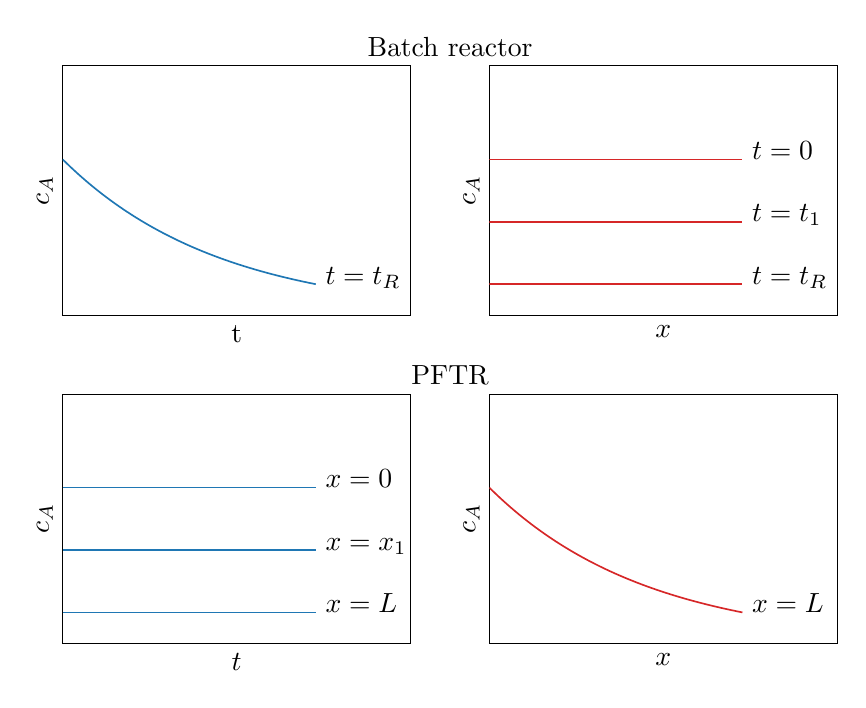
\begin{tikzpicture}

\definecolor{color0}{rgb}{0.12156862745098,0.466666666666667,0.705882352941177}
\definecolor{color1}{rgb}{0.83921568627451,0.152941176470588,0.156862745098039}

\begin{groupplot}[group style={
                group name=my plots,
                group size=2 by 2,
                vertical sep=1cm
            }]
\nextgroupplot[
height=4.75cm,
ylabel near ticks,
xlabel near ticks,
xtick=\empty,
ytick=\empty,
width=6cm,
xlabel={t},
xmin=0, xmax=2.75,
ylabel={\(\displaystyle c_A\)},
ymin=0, ymax=8
]
\addplot [semithick, color0]
table {%
0 5
0.0202020202020202 4.91937241196215
0.0404040404040404 4.84004498551486
0.0606060606060606 4.7619967548795
0.0808080808080808 4.6852070923615
0.101010101010101 4.60965570289851
0.121212121212121 4.53532261869659
0.141414141414141 4.46218819395278
0.161616161616162 4.3902330996629
0.181818181818182 4.31943831851295
0.202020202020202 4.24978513985296
0.222222222222222 4.18125515475187
0.242424242424242 4.11383025113217
0.262626262626263 4.04749260898298
0.282828282828283 3.98222469565032
0.303030303030303 3.91800926120331
0.323232323232323 3.85482933387515
0.343434343434343 3.79266821557757
0.363636363636364 3.7315094774876
0.383838383838384 3.67133695570556
0.404040404040404 3.612134746983
0.424242424242424 3.55388720451961
0.444444444444444 3.49657893382781
0.464646464646465 3.44019478866411
0.484848484848485 3.38471986702604
0.505050505050505 3.33013950721362
0.525252525252525 3.27643928395438
0.545454545454546 3.22360500459084
0.565656565656566 3.17162270532945
0.585858585858586 3.12047864755009
0.606060606060606 3.07015931417498
0.626262626262626 3.0206514060962
0.646464646464647 2.97194183866087
0.666666666666667 2.92401773821287
0.686868686868687 2.87686643869047
0.707070707070707 2.83047547827874
0.727272727272727 2.78483259611596
0.747474747474748 2.73992572905315
0.767676767676768 2.69574300846587
0.787878787878788 2.65227275711737
0.808080808080808 2.60950348607239
0.828282828282828 2.56742389166072
0.848484848484849 2.52602285248965
0.868686868686869 2.4852894265047
0.888888888888889 2.44521284809769
0.909090909090909 2.40578252526143
0.929292929292929 2.36698803679034
0.94949494949495 2.32881912952617
0.96969696969697 2.29126571564815
0.98989898989899 2.25431787000685
1.01010101010101 2.21796582750099
1.03030303030303 2.18219998049663
1.05050505050505 2.14701087628789
1.07070707070707 2.11238921459867
1.09090909090909 2.07832584512462
1.11111111111111 2.04481176511479
1.13131313131313 2.01183811699227
1.15151515151515 1.97939618601313
1.17171717171717 1.94747739796321
1.19191919191919 1.91607331689201
1.21212121212121 1.88517564288307
1.23232323232323 1.8547762098604
1.25252525252525 1.82486698343019
1.27272727272727 1.79544005875742
1.29292929292929 1.76648765847659
1.31313131313131 1.73800213063627
1.33333333333333 1.7099759466767
1.35353535353535 1.68240169944004
1.37373737373737 1.65527210121271
1.39393939393939 1.62857998179929
1.41414141414141 1.60231828662745
1.43434343434343 1.5764800748835
1.45454545454545 1.55105851767799
1.47474747474747 1.5260468962408
1.4949494949495 1.50143860014549
1.51515151515152 1.47722712556216
1.53535353535354 1.45340607353852
1.55555555555556 1.42996914830873
1.57575757575758 1.40691015562939
1.5959595959596 1.38422300114252
1.61616161616162 1.36190168876479
1.63636363636364 1.33994031910284
1.65656565656566 1.31833308789405
1.67676767676768 1.29707428447257
1.6969696969697 1.27615829025999
1.71717171717172 1.25557957728035
1.73737373737374 1.23533270669921
1.75757575757576 1.21541232738612
1.77777777777778 1.1958131745004
1.7979797979798 1.17653006809963
1.81818181818182 1.15755791177065
1.83838383838384 1.13889169128261
1.85858585858586 1.12052647326172
1.87878787878788 1.10245740388739
1.8989898989899 1.08467970760941
1.91919191919192 1.06718868588578
1.93939393939394 1.04997971594093
1.95959595959596 1.03304824954393
1.97979797979798 1.01638981180644
2 1
};
\draw (axis cs:2,1) node[
  anchor=base west,
  text=black,
  rotate=0.0
]{$t = t_R$};

\nextgroupplot[
height=4.75cm,
ylabel near ticks,
xlabel near ticks,
xtick=\empty,
ytick=\empty,
width=6cm,
xlabel={\(\displaystyle x\)},
xmin=0, xmax=2.75,
ylabel={\(\displaystyle c_A\)},
ymin=0, ymax=8
]
\addplot [semithick, color1]
table {%
0 5
0.0202020202020202 5
0.0404040404040404 5
0.0606060606060606 5
0.0808080808080808 5
0.101010101010101 5
0.121212121212121 5
0.141414141414141 5
0.161616161616162 5
0.181818181818182 5
0.202020202020202 5
0.222222222222222 5
0.242424242424242 5
0.262626262626263 5
0.282828282828283 5
0.303030303030303 5
0.323232323232323 5
0.343434343434343 5
0.363636363636364 5
0.383838383838384 5
0.404040404040404 5
0.424242424242424 5
0.444444444444444 5
0.464646464646465 5
0.484848484848485 5
0.505050505050505 5
0.525252525252525 5
0.545454545454546 5
0.565656565656566 5
0.585858585858586 5
0.606060606060606 5
0.626262626262626 5
0.646464646464647 5
0.666666666666667 5
0.686868686868687 5
0.707070707070707 5
0.727272727272727 5
0.747474747474748 5
0.767676767676768 5
0.787878787878788 5
0.808080808080808 5
0.828282828282828 5
0.848484848484849 5
0.868686868686869 5
0.888888888888889 5
0.909090909090909 5
0.929292929292929 5
0.94949494949495 5
0.96969696969697 5
0.98989898989899 5
1.01010101010101 5
1.03030303030303 5
1.05050505050505 5
1.07070707070707 5
1.09090909090909 5
1.11111111111111 5
1.13131313131313 5
1.15151515151515 5
1.17171717171717 5
1.19191919191919 5
1.21212121212121 5
1.23232323232323 5
1.25252525252525 5
1.27272727272727 5
1.29292929292929 5
1.31313131313131 5
1.33333333333333 5
1.35353535353535 5
1.37373737373737 5
1.39393939393939 5
1.41414141414141 5
1.43434343434343 5
1.45454545454545 5
1.47474747474747 5
1.4949494949495 5
1.51515151515152 5
1.53535353535354 5
1.55555555555556 5
1.57575757575758 5
1.5959595959596 5
1.61616161616162 5
1.63636363636364 5
1.65656565656566 5
1.67676767676768 5
1.6969696969697 5
1.71717171717172 5
1.73737373737374 5
1.75757575757576 5
1.77777777777778 5
1.7979797979798 5
1.81818181818182 5
1.83838383838384 5
1.85858585858586 5
1.87878787878788 5
1.8989898989899 5
1.91919191919192 5
1.93939393939394 5
1.95959595959596 5
1.97979797979798 5
2 5
};
\addplot [semithick, color1]
table {%
0 3
0.0202020202020202 3
0.0404040404040404 3
0.0606060606060606 3
0.0808080808080808 3
0.101010101010101 3
0.121212121212121 3
0.141414141414141 3
0.161616161616162 3
0.181818181818182 3
0.202020202020202 3
0.222222222222222 3
0.242424242424242 3
0.262626262626263 3
0.282828282828283 3
0.303030303030303 3
0.323232323232323 3
0.343434343434343 3
0.363636363636364 3
0.383838383838384 3
0.404040404040404 3
0.424242424242424 3
0.444444444444444 3
0.464646464646465 3
0.484848484848485 3
0.505050505050505 3
0.525252525252525 3
0.545454545454546 3
0.565656565656566 3
0.585858585858586 3
0.606060606060606 3
0.626262626262626 3
0.646464646464647 3
0.666666666666667 3
0.686868686868687 3
0.707070707070707 3
0.727272727272727 3
0.747474747474748 3
0.767676767676768 3
0.787878787878788 3
0.808080808080808 3
0.828282828282828 3
0.848484848484849 3
0.868686868686869 3
0.888888888888889 3
0.909090909090909 3
0.929292929292929 3
0.94949494949495 3
0.96969696969697 3
0.98989898989899 3
1.01010101010101 3
1.03030303030303 3
1.05050505050505 3
1.07070707070707 3
1.09090909090909 3
1.11111111111111 3
1.13131313131313 3
1.15151515151515 3
1.17171717171717 3
1.19191919191919 3
1.21212121212121 3
1.23232323232323 3
1.25252525252525 3
1.27272727272727 3
1.29292929292929 3
1.31313131313131 3
1.33333333333333 3
1.35353535353535 3
1.37373737373737 3
1.39393939393939 3
1.41414141414141 3
1.43434343434343 3
1.45454545454545 3
1.47474747474747 3
1.4949494949495 3
1.51515151515152 3
1.53535353535354 3
1.55555555555556 3
1.57575757575758 3
1.5959595959596 3
1.61616161616162 3
1.63636363636364 3
1.65656565656566 3
1.67676767676768 3
1.6969696969697 3
1.71717171717172 3
1.73737373737374 3
1.75757575757576 3
1.77777777777778 3
1.7979797979798 3
1.81818181818182 3
1.83838383838384 3
1.85858585858586 3
1.87878787878788 3
1.8989898989899 3
1.91919191919192 3
1.93939393939394 3
1.95959595959596 3
1.97979797979798 3
2 3
};
\addplot [semithick, color1]
table {%
0 1
0.0202020202020202 1
0.0404040404040404 1
0.0606060606060606 1
0.0808080808080808 1
0.101010101010101 1
0.121212121212121 1
0.141414141414141 1
0.161616161616162 1
0.181818181818182 1
0.202020202020202 1
0.222222222222222 1
0.242424242424242 1
0.262626262626263 1
0.282828282828283 1
0.303030303030303 1
0.323232323232323 1
0.343434343434343 1
0.363636363636364 1
0.383838383838384 1
0.404040404040404 1
0.424242424242424 1
0.444444444444444 1
0.464646464646465 1
0.484848484848485 1
0.505050505050505 1
0.525252525252525 1
0.545454545454546 1
0.565656565656566 1
0.585858585858586 1
0.606060606060606 1
0.626262626262626 1
0.646464646464647 1
0.666666666666667 1
0.686868686868687 1
0.707070707070707 1
0.727272727272727 1
0.747474747474748 1
0.767676767676768 1
0.787878787878788 1
0.808080808080808 1
0.828282828282828 1
0.848484848484849 1
0.868686868686869 1
0.888888888888889 1
0.909090909090909 1
0.929292929292929 1
0.94949494949495 1
0.96969696969697 1
0.98989898989899 1
1.01010101010101 1
1.03030303030303 1
1.05050505050505 1
1.07070707070707 1
1.09090909090909 1
1.11111111111111 1
1.13131313131313 1
1.15151515151515 1
1.17171717171717 1
1.19191919191919 1
1.21212121212121 1
1.23232323232323 1
1.25252525252525 1
1.27272727272727 1
1.29292929292929 1
1.31313131313131 1
1.33333333333333 1
1.35353535353535 1
1.37373737373737 1
1.39393939393939 1
1.41414141414141 1
1.43434343434343 1
1.45454545454545 1
1.47474747474747 1
1.4949494949495 1
1.51515151515152 1
1.53535353535354 1
1.55555555555556 1
1.57575757575758 1
1.5959595959596 1
1.61616161616162 1
1.63636363636364 1
1.65656565656566 1
1.67676767676768 1
1.6969696969697 1
1.71717171717172 1
1.73737373737374 1
1.75757575757576 1
1.77777777777778 1
1.7979797979798 1
1.81818181818182 1
1.83838383838384 1
1.85858585858586 1
1.87878787878788 1
1.8989898989899 1
1.91919191919192 1
1.93939393939394 1
1.95959595959596 1
1.97979797979798 1
2 1
};
\draw (axis cs:2,5) node[
  anchor=base west,
  text=black,
  rotate=0.0
]{$t = 0$};
\draw (axis cs:2,3) node[
  anchor=base west,
  text=black,
  rotate=0.0
]{$t = t_1$};
\draw (axis cs:2,1) node[
  anchor=base west,
  text=black,
  rotate=0.0
]{$t = t_R$};

\nextgroupplot[
height=4.75cm,
ylabel near ticks,
xlabel near ticks,
xtick=\empty,
ytick=\empty,
width=6cm,
xlabel={\(\displaystyle t\)},
xmin=0, xmax=2.75,
ylabel={\(\displaystyle c_A\)},
ymin=0, ymax=8
]
\addplot [semithick, color0]
table {%
0 5
0.0202020202020202 5
0.0404040404040404 5
0.0606060606060606 5
0.0808080808080808 5
0.101010101010101 5
0.121212121212121 5
0.141414141414141 5
0.161616161616162 5
0.181818181818182 5
0.202020202020202 5
0.222222222222222 5
0.242424242424242 5
0.262626262626263 5
0.282828282828283 5
0.303030303030303 5
0.323232323232323 5
0.343434343434343 5
0.363636363636364 5
0.383838383838384 5
0.404040404040404 5
0.424242424242424 5
0.444444444444444 5
0.464646464646465 5
0.484848484848485 5
0.505050505050505 5
0.525252525252525 5
0.545454545454546 5
0.565656565656566 5
0.585858585858586 5
0.606060606060606 5
0.626262626262626 5
0.646464646464647 5
0.666666666666667 5
0.686868686868687 5
0.707070707070707 5
0.727272727272727 5
0.747474747474748 5
0.767676767676768 5
0.787878787878788 5
0.808080808080808 5
0.828282828282828 5
0.848484848484849 5
0.868686868686869 5
0.888888888888889 5
0.909090909090909 5
0.929292929292929 5
0.94949494949495 5
0.96969696969697 5
0.98989898989899 5
1.01010101010101 5
1.03030303030303 5
1.05050505050505 5
1.07070707070707 5
1.09090909090909 5
1.11111111111111 5
1.13131313131313 5
1.15151515151515 5
1.17171717171717 5
1.19191919191919 5
1.21212121212121 5
1.23232323232323 5
1.25252525252525 5
1.27272727272727 5
1.29292929292929 5
1.31313131313131 5
1.33333333333333 5
1.35353535353535 5
1.37373737373737 5
1.39393939393939 5
1.41414141414141 5
1.43434343434343 5
1.45454545454545 5
1.47474747474747 5
1.4949494949495 5
1.51515151515152 5
1.53535353535354 5
1.55555555555556 5
1.57575757575758 5
1.5959595959596 5
1.61616161616162 5
1.63636363636364 5
1.65656565656566 5
1.67676767676768 5
1.6969696969697 5
1.71717171717172 5
1.73737373737374 5
1.75757575757576 5
1.77777777777778 5
1.7979797979798 5
1.81818181818182 5
1.83838383838384 5
1.85858585858586 5
1.87878787878788 5
1.8989898989899 5
1.91919191919192 5
1.93939393939394 5
1.95959595959596 5
1.97979797979798 5
2 5
};
\addplot [semithick, color0]
table {%
0 3
0.0202020202020202 3
0.0404040404040404 3
0.0606060606060606 3
0.0808080808080808 3
0.101010101010101 3
0.121212121212121 3
0.141414141414141 3
0.161616161616162 3
0.181818181818182 3
0.202020202020202 3
0.222222222222222 3
0.242424242424242 3
0.262626262626263 3
0.282828282828283 3
0.303030303030303 3
0.323232323232323 3
0.343434343434343 3
0.363636363636364 3
0.383838383838384 3
0.404040404040404 3
0.424242424242424 3
0.444444444444444 3
0.464646464646465 3
0.484848484848485 3
0.505050505050505 3
0.525252525252525 3
0.545454545454546 3
0.565656565656566 3
0.585858585858586 3
0.606060606060606 3
0.626262626262626 3
0.646464646464647 3
0.666666666666667 3
0.686868686868687 3
0.707070707070707 3
0.727272727272727 3
0.747474747474748 3
0.767676767676768 3
0.787878787878788 3
0.808080808080808 3
0.828282828282828 3
0.848484848484849 3
0.868686868686869 3
0.888888888888889 3
0.909090909090909 3
0.929292929292929 3
0.94949494949495 3
0.96969696969697 3
0.98989898989899 3
1.01010101010101 3
1.03030303030303 3
1.05050505050505 3
1.07070707070707 3
1.09090909090909 3
1.11111111111111 3
1.13131313131313 3
1.15151515151515 3
1.17171717171717 3
1.19191919191919 3
1.21212121212121 3
1.23232323232323 3
1.25252525252525 3
1.27272727272727 3
1.29292929292929 3
1.31313131313131 3
1.33333333333333 3
1.35353535353535 3
1.37373737373737 3
1.39393939393939 3
1.41414141414141 3
1.43434343434343 3
1.45454545454545 3
1.47474747474747 3
1.4949494949495 3
1.51515151515152 3
1.53535353535354 3
1.55555555555556 3
1.57575757575758 3
1.5959595959596 3
1.61616161616162 3
1.63636363636364 3
1.65656565656566 3
1.67676767676768 3
1.6969696969697 3
1.71717171717172 3
1.73737373737374 3
1.75757575757576 3
1.77777777777778 3
1.7979797979798 3
1.81818181818182 3
1.83838383838384 3
1.85858585858586 3
1.87878787878788 3
1.8989898989899 3
1.91919191919192 3
1.93939393939394 3
1.95959595959596 3
1.97979797979798 3
2 3
};
\addplot [semithick, color0]
table {%
0 1
0.0202020202020202 1
0.0404040404040404 1
0.0606060606060606 1
0.0808080808080808 1
0.101010101010101 1
0.121212121212121 1
0.141414141414141 1
0.161616161616162 1
0.181818181818182 1
0.202020202020202 1
0.222222222222222 1
0.242424242424242 1
0.262626262626263 1
0.282828282828283 1
0.303030303030303 1
0.323232323232323 1
0.343434343434343 1
0.363636363636364 1
0.383838383838384 1
0.404040404040404 1
0.424242424242424 1
0.444444444444444 1
0.464646464646465 1
0.484848484848485 1
0.505050505050505 1
0.525252525252525 1
0.545454545454546 1
0.565656565656566 1
0.585858585858586 1
0.606060606060606 1
0.626262626262626 1
0.646464646464647 1
0.666666666666667 1
0.686868686868687 1
0.707070707070707 1
0.727272727272727 1
0.747474747474748 1
0.767676767676768 1
0.787878787878788 1
0.808080808080808 1
0.828282828282828 1
0.848484848484849 1
0.868686868686869 1
0.888888888888889 1
0.909090909090909 1
0.929292929292929 1
0.94949494949495 1
0.96969696969697 1
0.98989898989899 1
1.01010101010101 1
1.03030303030303 1
1.05050505050505 1
1.07070707070707 1
1.09090909090909 1
1.11111111111111 1
1.13131313131313 1
1.15151515151515 1
1.17171717171717 1
1.19191919191919 1
1.21212121212121 1
1.23232323232323 1
1.25252525252525 1
1.27272727272727 1
1.29292929292929 1
1.31313131313131 1
1.33333333333333 1
1.35353535353535 1
1.37373737373737 1
1.39393939393939 1
1.41414141414141 1
1.43434343434343 1
1.45454545454545 1
1.47474747474747 1
1.4949494949495 1
1.51515151515152 1
1.53535353535354 1
1.55555555555556 1
1.57575757575758 1
1.5959595959596 1
1.61616161616162 1
1.63636363636364 1
1.65656565656566 1
1.67676767676768 1
1.6969696969697 1
1.71717171717172 1
1.73737373737374 1
1.75757575757576 1
1.77777777777778 1
1.7979797979798 1
1.81818181818182 1
1.83838383838384 1
1.85858585858586 1
1.87878787878788 1
1.8989898989899 1
1.91919191919192 1
1.93939393939394 1
1.95959595959596 1
1.97979797979798 1
2 1
};
\draw (axis cs:2,5) node[
  anchor=base west,
  text=black,
  rotate=0.0
]{$x = 0$};
\draw (axis cs:2,3) node[
  anchor=base west,
  text=black,
  rotate=0.0
]{$x = x_1$};
\draw (axis cs:2,1) node[
  anchor=base west,
  text=black,
  rotate=0.0
]{$x = L$};

\nextgroupplot[
height=4.75cm,
ylabel near ticks,
xlabel near ticks,
xtick=\empty,
ytick=\empty,
width=6cm,
xlabel={\(\displaystyle x\)},
xmin=0, xmax=2.75,
ylabel={\(\displaystyle c_A\)},
ymin=0, ymax=8
]
\addplot [semithick, color1]
table {%
0 5
0.0202020202020202 4.91937241196215
0.0404040404040404 4.84004498551486
0.0606060606060606 4.7619967548795
0.0808080808080808 4.6852070923615
0.101010101010101 4.60965570289851
0.121212121212121 4.53532261869659
0.141414141414141 4.46218819395278
0.161616161616162 4.3902330996629
0.181818181818182 4.31943831851295
0.202020202020202 4.24978513985296
0.222222222222222 4.18125515475187
0.242424242424242 4.11383025113217
0.262626262626263 4.04749260898298
0.282828282828283 3.98222469565032
0.303030303030303 3.91800926120331
0.323232323232323 3.85482933387515
0.343434343434343 3.79266821557757
0.363636363636364 3.7315094774876
0.383838383838384 3.67133695570556
0.404040404040404 3.612134746983
0.424242424242424 3.55388720451961
0.444444444444444 3.49657893382781
0.464646464646465 3.44019478866411
0.484848484848485 3.38471986702604
0.505050505050505 3.33013950721362
0.525252525252525 3.27643928395438
0.545454545454546 3.22360500459084
0.565656565656566 3.17162270532945
0.585858585858586 3.12047864755009
0.606060606060606 3.07015931417498
0.626262626262626 3.0206514060962
0.646464646464647 2.97194183866087
0.666666666666667 2.92401773821287
0.686868686868687 2.87686643869047
0.707070707070707 2.83047547827874
0.727272727272727 2.78483259611596
0.747474747474748 2.73992572905315
0.767676767676768 2.69574300846587
0.787878787878788 2.65227275711737
0.808080808080808 2.60950348607239
0.828282828282828 2.56742389166072
0.848484848484849 2.52602285248965
0.868686868686869 2.4852894265047
0.888888888888889 2.44521284809769
0.909090909090909 2.40578252526143
0.929292929292929 2.36698803679034
0.94949494949495 2.32881912952617
0.96969696969697 2.29126571564815
0.98989898989899 2.25431787000685
1.01010101010101 2.21796582750099
1.03030303030303 2.18219998049663
1.05050505050505 2.14701087628789
1.07070707070707 2.11238921459867
1.09090909090909 2.07832584512462
1.11111111111111 2.04481176511479
1.13131313131313 2.01183811699227
1.15151515151515 1.97939618601313
1.17171717171717 1.94747739796321
1.19191919191919 1.91607331689201
1.21212121212121 1.88517564288307
1.23232323232323 1.8547762098604
1.25252525252525 1.82486698343019
1.27272727272727 1.79544005875742
1.29292929292929 1.76648765847659
1.31313131313131 1.73800213063627
1.33333333333333 1.7099759466767
1.35353535353535 1.68240169944004
1.37373737373737 1.65527210121271
1.39393939393939 1.62857998179929
1.41414141414141 1.60231828662745
1.43434343434343 1.5764800748835
1.45454545454545 1.55105851767799
1.47474747474747 1.5260468962408
1.4949494949495 1.50143860014549
1.51515151515152 1.47722712556216
1.53535353535354 1.45340607353852
1.55555555555556 1.42996914830873
1.57575757575758 1.40691015562939
1.5959595959596 1.38422300114252
1.61616161616162 1.36190168876479
1.63636363636364 1.33994031910284
1.65656565656566 1.31833308789405
1.67676767676768 1.29707428447257
1.6969696969697 1.27615829025999
1.71717171717172 1.25557957728035
1.73737373737374 1.23533270669921
1.75757575757576 1.21541232738612
1.77777777777778 1.1958131745004
1.7979797979798 1.17653006809963
1.81818181818182 1.15755791177065
1.83838383838384 1.13889169128261
1.85858585858586 1.12052647326172
1.87878787878788 1.10245740388739
1.8989898989899 1.08467970760941
1.91919191919192 1.06718868588578
1.93939393939394 1.04997971594093
1.95959595959596 1.03304824954393
1.97979797979798 1.01638981180644
2 1
};
\draw (axis cs:2,1) node[
  anchor=base west,
  text=black,
  rotate=0.0
]{$x = L$};
\end{groupplot}
\node[anchor=south] at ($(my plots c1r1.north east)!0.5!(my plots c2r1.north west)$){Batch reactor};
\node[anchor=south] at ($(my plots c1r2.north east)!0.5!(my plots c2r2.north west)$){PFTR};
\end{tikzpicture}

\end{center}
Time and location dependence on temperature:
\begin{center}
% This file was created by tikzplotlib v0.9.8.
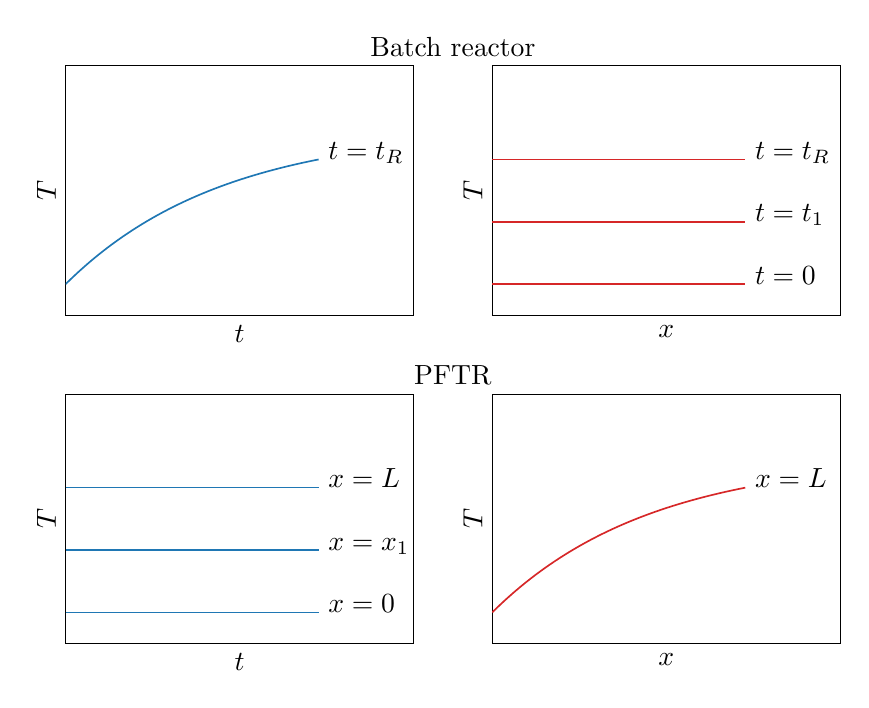
\begin{tikzpicture}

\definecolor{color0}{rgb}{0.12156862745098,0.466666666666667,0.705882352941177}
\definecolor{color1}{rgb}{0.83921568627451,0.152941176470588,0.156862745098039}

\begin{groupplot}[group style={
                group name=my plots,
                group size=2 by 2,
                vertical sep=1cm
            }]
\nextgroupplot[
height=4.75cm,
ylabel near ticks,
xlabel near ticks,
xtick=\empty,
ytick=\empty,
width=6cm,
xlabel={\(\displaystyle t\)},
xmin=0, xmax=2.75,
ylabel={\(\displaystyle T\)},
ymin=0, ymax=8
]
\addplot [semithick, color0]
table {%
0 1
0.0202020202020202 1.08062758803785
0.0404040404040404 1.15995501448514
0.0606060606060606 1.2380032451205
0.0808080808080808 1.3147929076385
0.101010101010101 1.39034429710149
0.121212121212121 1.46467738130341
0.141414141414141 1.53781180604722
0.161616161616162 1.6097669003371
0.181818181818182 1.68056168148705
0.202020202020202 1.75021486014704
0.222222222222222 1.81874484524813
0.242424242424242 1.88616974886783
0.262626262626263 1.95250739101702
0.282828282828283 2.01777530434968
0.303030303030303 2.08199073879669
0.323232323232323 2.14517066612485
0.343434343434343 2.20733178442243
0.363636363636364 2.2684905225124
0.383838383838384 2.32866304429444
0.404040404040404 2.387865253017
0.424242424242424 2.44611279548039
0.444444444444444 2.50342106617219
0.464646464646465 2.55980521133589
0.484848484848485 2.61528013297396
0.505050505050505 2.66986049278638
0.525252525252525 2.72356071604562
0.545454545454546 2.77639499540916
0.565656565656566 2.82837729467055
0.585858585858586 2.87952135244991
0.606060606060606 2.92984068582502
0.626262626262626 2.9793485939038
0.646464646464647 3.02805816133913
0.666666666666667 3.07598226178713
0.686868686868687 3.12313356130953
0.707070707070707 3.16952452172126
0.727272727272727 3.21516740388404
0.747474747474748 3.26007427094685
0.767676767676768 3.30425699153413
0.787878787878788 3.34772724288263
0.808080808080808 3.39049651392761
0.828282828282828 3.43257610833928
0.848484848484849 3.47397714751035
0.868686868686869 3.5147105734953
0.888888888888889 3.55478715190231
0.909090909090909 3.59421747473857
0.929292929292929 3.63301196320966
0.94949494949495 3.67118087047383
0.96969696969697 3.70873428435185
0.98989898989899 3.74568212999315
1.01010101010101 3.78203417249901
1.03030303030303 3.81780001950337
1.05050505050505 3.85298912371211
1.07070707070707 3.88761078540133
1.09090909090909 3.92167415487538
1.11111111111111 3.95518823488521
1.13131313131313 3.98816188300774
1.15151515151515 4.02060381398687
1.17171717171717 4.05252260203679
1.19191919191919 4.08392668310799
1.21212121212121 4.11482435711692
1.23232323232323 4.1452237901396
1.25252525252525 4.17513301656981
1.27272727272727 4.20455994124258
1.29292929292929 4.23351234152341
1.31313131313131 4.26199786936373
1.33333333333333 4.2900240533233
1.35353535353535 4.31759830055996
1.37373737373737 4.34472789878729
1.39393939393939 4.37142001820071
1.41414141414141 4.39768171337255
1.43434343434343 4.4235199251165
1.45454545454545 4.44894148232201
1.47474747474747 4.4739531037592
1.4949494949495 4.49856139985451
1.51515151515152 4.52277287443784
1.53535353535354 4.54659392646148
1.55555555555556 4.57003085169127
1.57575757575758 4.59308984437061
1.5959595959596 4.61577699885748
1.61616161616162 4.6380983112352
1.63636363636364 4.66005968089716
1.65656565656566 4.68166691210595
1.67676767676768 4.70292571552743
1.6969696969697 4.72384170974001
1.71717171717172 4.74442042271965
1.73737373737374 4.76466729330079
1.75757575757576 4.78458767261387
1.77777777777778 4.8041868254996
1.7979797979798 4.82346993190037
1.81818181818182 4.84244208822935
1.83838383838384 4.86110830871739
1.85858585858586 4.87947352673828
1.87878787878788 4.89754259611261
1.8989898989899 4.91532029239059
1.91919191919192 4.93281131411422
1.93939393939394 4.95002028405907
1.95959595959596 4.96695175045607
1.97979797979798 4.98361018819356
2 5
};
\draw (axis cs:2,5) node[
  anchor=base west,
  text=black,
  rotate=0.0
]{$t = t_R$};

\nextgroupplot[
height=4.75cm,
ylabel near ticks,
xlabel near ticks,
xtick=\empty,
ytick=\empty,
width=6cm,
xlabel={\(\displaystyle x\)},
xmin=0, xmax=2.75,
ylabel={\(\displaystyle T\)},
ymin=0, ymax=8
]
\addplot [semithick, color1]
table {%
0 5
0.0202020202020202 5
0.0404040404040404 5
0.0606060606060606 5
0.0808080808080808 5
0.101010101010101 5
0.121212121212121 5
0.141414141414141 5
0.161616161616162 5
0.181818181818182 5
0.202020202020202 5
0.222222222222222 5
0.242424242424242 5
0.262626262626263 5
0.282828282828283 5
0.303030303030303 5
0.323232323232323 5
0.343434343434343 5
0.363636363636364 5
0.383838383838384 5
0.404040404040404 5
0.424242424242424 5
0.444444444444444 5
0.464646464646465 5
0.484848484848485 5
0.505050505050505 5
0.525252525252525 5
0.545454545454546 5
0.565656565656566 5
0.585858585858586 5
0.606060606060606 5
0.626262626262626 5
0.646464646464647 5
0.666666666666667 5
0.686868686868687 5
0.707070707070707 5
0.727272727272727 5
0.747474747474748 5
0.767676767676768 5
0.787878787878788 5
0.808080808080808 5
0.828282828282828 5
0.848484848484849 5
0.868686868686869 5
0.888888888888889 5
0.909090909090909 5
0.929292929292929 5
0.94949494949495 5
0.96969696969697 5
0.98989898989899 5
1.01010101010101 5
1.03030303030303 5
1.05050505050505 5
1.07070707070707 5
1.09090909090909 5
1.11111111111111 5
1.13131313131313 5
1.15151515151515 5
1.17171717171717 5
1.19191919191919 5
1.21212121212121 5
1.23232323232323 5
1.25252525252525 5
1.27272727272727 5
1.29292929292929 5
1.31313131313131 5
1.33333333333333 5
1.35353535353535 5
1.37373737373737 5
1.39393939393939 5
1.41414141414141 5
1.43434343434343 5
1.45454545454545 5
1.47474747474747 5
1.4949494949495 5
1.51515151515152 5
1.53535353535354 5
1.55555555555556 5
1.57575757575758 5
1.5959595959596 5
1.61616161616162 5
1.63636363636364 5
1.65656565656566 5
1.67676767676768 5
1.6969696969697 5
1.71717171717172 5
1.73737373737374 5
1.75757575757576 5
1.77777777777778 5
1.7979797979798 5
1.81818181818182 5
1.83838383838384 5
1.85858585858586 5
1.87878787878788 5
1.8989898989899 5
1.91919191919192 5
1.93939393939394 5
1.95959595959596 5
1.97979797979798 5
2 5
};
\addplot [semithick, color1]
table {%
0 3
0.0202020202020202 3
0.0404040404040404 3
0.0606060606060606 3
0.0808080808080808 3
0.101010101010101 3
0.121212121212121 3
0.141414141414141 3
0.161616161616162 3
0.181818181818182 3
0.202020202020202 3
0.222222222222222 3
0.242424242424242 3
0.262626262626263 3
0.282828282828283 3
0.303030303030303 3
0.323232323232323 3
0.343434343434343 3
0.363636363636364 3
0.383838383838384 3
0.404040404040404 3
0.424242424242424 3
0.444444444444444 3
0.464646464646465 3
0.484848484848485 3
0.505050505050505 3
0.525252525252525 3
0.545454545454546 3
0.565656565656566 3
0.585858585858586 3
0.606060606060606 3
0.626262626262626 3
0.646464646464647 3
0.666666666666667 3
0.686868686868687 3
0.707070707070707 3
0.727272727272727 3
0.747474747474748 3
0.767676767676768 3
0.787878787878788 3
0.808080808080808 3
0.828282828282828 3
0.848484848484849 3
0.868686868686869 3
0.888888888888889 3
0.909090909090909 3
0.929292929292929 3
0.94949494949495 3
0.96969696969697 3
0.98989898989899 3
1.01010101010101 3
1.03030303030303 3
1.05050505050505 3
1.07070707070707 3
1.09090909090909 3
1.11111111111111 3
1.13131313131313 3
1.15151515151515 3
1.17171717171717 3
1.19191919191919 3
1.21212121212121 3
1.23232323232323 3
1.25252525252525 3
1.27272727272727 3
1.29292929292929 3
1.31313131313131 3
1.33333333333333 3
1.35353535353535 3
1.37373737373737 3
1.39393939393939 3
1.41414141414141 3
1.43434343434343 3
1.45454545454545 3
1.47474747474747 3
1.4949494949495 3
1.51515151515152 3
1.53535353535354 3
1.55555555555556 3
1.57575757575758 3
1.5959595959596 3
1.61616161616162 3
1.63636363636364 3
1.65656565656566 3
1.67676767676768 3
1.6969696969697 3
1.71717171717172 3
1.73737373737374 3
1.75757575757576 3
1.77777777777778 3
1.7979797979798 3
1.81818181818182 3
1.83838383838384 3
1.85858585858586 3
1.87878787878788 3
1.8989898989899 3
1.91919191919192 3
1.93939393939394 3
1.95959595959596 3
1.97979797979798 3
2 3
};
\addplot [semithick, color1]
table {%
0 1
0.0202020202020202 1
0.0404040404040404 1
0.0606060606060606 1
0.0808080808080808 1
0.101010101010101 1
0.121212121212121 1
0.141414141414141 1
0.161616161616162 1
0.181818181818182 1
0.202020202020202 1
0.222222222222222 1
0.242424242424242 1
0.262626262626263 1
0.282828282828283 1
0.303030303030303 1
0.323232323232323 1
0.343434343434343 1
0.363636363636364 1
0.383838383838384 1
0.404040404040404 1
0.424242424242424 1
0.444444444444444 1
0.464646464646465 1
0.484848484848485 1
0.505050505050505 1
0.525252525252525 1
0.545454545454546 1
0.565656565656566 1
0.585858585858586 1
0.606060606060606 1
0.626262626262626 1
0.646464646464647 1
0.666666666666667 1
0.686868686868687 1
0.707070707070707 1
0.727272727272727 1
0.747474747474748 1
0.767676767676768 1
0.787878787878788 1
0.808080808080808 1
0.828282828282828 1
0.848484848484849 1
0.868686868686869 1
0.888888888888889 1
0.909090909090909 1
0.929292929292929 1
0.94949494949495 1
0.96969696969697 1
0.98989898989899 1
1.01010101010101 1
1.03030303030303 1
1.05050505050505 1
1.07070707070707 1
1.09090909090909 1
1.11111111111111 1
1.13131313131313 1
1.15151515151515 1
1.17171717171717 1
1.19191919191919 1
1.21212121212121 1
1.23232323232323 1
1.25252525252525 1
1.27272727272727 1
1.29292929292929 1
1.31313131313131 1
1.33333333333333 1
1.35353535353535 1
1.37373737373737 1
1.39393939393939 1
1.41414141414141 1
1.43434343434343 1
1.45454545454545 1
1.47474747474747 1
1.4949494949495 1
1.51515151515152 1
1.53535353535354 1
1.55555555555556 1
1.57575757575758 1
1.5959595959596 1
1.61616161616162 1
1.63636363636364 1
1.65656565656566 1
1.67676767676768 1
1.6969696969697 1
1.71717171717172 1
1.73737373737374 1
1.75757575757576 1
1.77777777777778 1
1.7979797979798 1
1.81818181818182 1
1.83838383838384 1
1.85858585858586 1
1.87878787878788 1
1.8989898989899 1
1.91919191919192 1
1.93939393939394 1
1.95959595959596 1
1.97979797979798 1
2 1
};
\draw (axis cs:2,5) node[
  anchor=base west,
  text=black,
  rotate=0.0
]{$t = t_R$};
\draw (axis cs:2,3) node[
  anchor=base west,
  text=black,
  rotate=0.0
]{$t = t_1$};
\draw (axis cs:2,1) node[
  anchor=base west,
  text=black,
  rotate=0.0
]{$t = 0$};

\nextgroupplot[
height=4.75cm,
ylabel near ticks,
xlabel near ticks,
xtick=\empty,
ytick=\empty,
width=6cm,
xlabel={\(\displaystyle t\)},
xmin=0, xmax=2.75,
ylabel={\(\displaystyle T\)},
ymin=0, ymax=8
]
\addplot [semithick, color0]
table {%
0 5
0.0202020202020202 5
0.0404040404040404 5
0.0606060606060606 5
0.0808080808080808 5
0.101010101010101 5
0.121212121212121 5
0.141414141414141 5
0.161616161616162 5
0.181818181818182 5
0.202020202020202 5
0.222222222222222 5
0.242424242424242 5
0.262626262626263 5
0.282828282828283 5
0.303030303030303 5
0.323232323232323 5
0.343434343434343 5
0.363636363636364 5
0.383838383838384 5
0.404040404040404 5
0.424242424242424 5
0.444444444444444 5
0.464646464646465 5
0.484848484848485 5
0.505050505050505 5
0.525252525252525 5
0.545454545454546 5
0.565656565656566 5
0.585858585858586 5
0.606060606060606 5
0.626262626262626 5
0.646464646464647 5
0.666666666666667 5
0.686868686868687 5
0.707070707070707 5
0.727272727272727 5
0.747474747474748 5
0.767676767676768 5
0.787878787878788 5
0.808080808080808 5
0.828282828282828 5
0.848484848484849 5
0.868686868686869 5
0.888888888888889 5
0.909090909090909 5
0.929292929292929 5
0.94949494949495 5
0.96969696969697 5
0.98989898989899 5
1.01010101010101 5
1.03030303030303 5
1.05050505050505 5
1.07070707070707 5
1.09090909090909 5
1.11111111111111 5
1.13131313131313 5
1.15151515151515 5
1.17171717171717 5
1.19191919191919 5
1.21212121212121 5
1.23232323232323 5
1.25252525252525 5
1.27272727272727 5
1.29292929292929 5
1.31313131313131 5
1.33333333333333 5
1.35353535353535 5
1.37373737373737 5
1.39393939393939 5
1.41414141414141 5
1.43434343434343 5
1.45454545454545 5
1.47474747474747 5
1.4949494949495 5
1.51515151515152 5
1.53535353535354 5
1.55555555555556 5
1.57575757575758 5
1.5959595959596 5
1.61616161616162 5
1.63636363636364 5
1.65656565656566 5
1.67676767676768 5
1.6969696969697 5
1.71717171717172 5
1.73737373737374 5
1.75757575757576 5
1.77777777777778 5
1.7979797979798 5
1.81818181818182 5
1.83838383838384 5
1.85858585858586 5
1.87878787878788 5
1.8989898989899 5
1.91919191919192 5
1.93939393939394 5
1.95959595959596 5
1.97979797979798 5
2 5
};
\addplot [semithick, color0]
table {%
0 3
0.0202020202020202 3
0.0404040404040404 3
0.0606060606060606 3
0.0808080808080808 3
0.101010101010101 3
0.121212121212121 3
0.141414141414141 3
0.161616161616162 3
0.181818181818182 3
0.202020202020202 3
0.222222222222222 3
0.242424242424242 3
0.262626262626263 3
0.282828282828283 3
0.303030303030303 3
0.323232323232323 3
0.343434343434343 3
0.363636363636364 3
0.383838383838384 3
0.404040404040404 3
0.424242424242424 3
0.444444444444444 3
0.464646464646465 3
0.484848484848485 3
0.505050505050505 3
0.525252525252525 3
0.545454545454546 3
0.565656565656566 3
0.585858585858586 3
0.606060606060606 3
0.626262626262626 3
0.646464646464647 3
0.666666666666667 3
0.686868686868687 3
0.707070707070707 3
0.727272727272727 3
0.747474747474748 3
0.767676767676768 3
0.787878787878788 3
0.808080808080808 3
0.828282828282828 3
0.848484848484849 3
0.868686868686869 3
0.888888888888889 3
0.909090909090909 3
0.929292929292929 3
0.94949494949495 3
0.96969696969697 3
0.98989898989899 3
1.01010101010101 3
1.03030303030303 3
1.05050505050505 3
1.07070707070707 3
1.09090909090909 3
1.11111111111111 3
1.13131313131313 3
1.15151515151515 3
1.17171717171717 3
1.19191919191919 3
1.21212121212121 3
1.23232323232323 3
1.25252525252525 3
1.27272727272727 3
1.29292929292929 3
1.31313131313131 3
1.33333333333333 3
1.35353535353535 3
1.37373737373737 3
1.39393939393939 3
1.41414141414141 3
1.43434343434343 3
1.45454545454545 3
1.47474747474747 3
1.4949494949495 3
1.51515151515152 3
1.53535353535354 3
1.55555555555556 3
1.57575757575758 3
1.5959595959596 3
1.61616161616162 3
1.63636363636364 3
1.65656565656566 3
1.67676767676768 3
1.6969696969697 3
1.71717171717172 3
1.73737373737374 3
1.75757575757576 3
1.77777777777778 3
1.7979797979798 3
1.81818181818182 3
1.83838383838384 3
1.85858585858586 3
1.87878787878788 3
1.8989898989899 3
1.91919191919192 3
1.93939393939394 3
1.95959595959596 3
1.97979797979798 3
2 3
};
\addplot [semithick, color0]
table {%
0 1
0.0202020202020202 1
0.0404040404040404 1
0.0606060606060606 1
0.0808080808080808 1
0.101010101010101 1
0.121212121212121 1
0.141414141414141 1
0.161616161616162 1
0.181818181818182 1
0.202020202020202 1
0.222222222222222 1
0.242424242424242 1
0.262626262626263 1
0.282828282828283 1
0.303030303030303 1
0.323232323232323 1
0.343434343434343 1
0.363636363636364 1
0.383838383838384 1
0.404040404040404 1
0.424242424242424 1
0.444444444444444 1
0.464646464646465 1
0.484848484848485 1
0.505050505050505 1
0.525252525252525 1
0.545454545454546 1
0.565656565656566 1
0.585858585858586 1
0.606060606060606 1
0.626262626262626 1
0.646464646464647 1
0.666666666666667 1
0.686868686868687 1
0.707070707070707 1
0.727272727272727 1
0.747474747474748 1
0.767676767676768 1
0.787878787878788 1
0.808080808080808 1
0.828282828282828 1
0.848484848484849 1
0.868686868686869 1
0.888888888888889 1
0.909090909090909 1
0.929292929292929 1
0.94949494949495 1
0.96969696969697 1
0.98989898989899 1
1.01010101010101 1
1.03030303030303 1
1.05050505050505 1
1.07070707070707 1
1.09090909090909 1
1.11111111111111 1
1.13131313131313 1
1.15151515151515 1
1.17171717171717 1
1.19191919191919 1
1.21212121212121 1
1.23232323232323 1
1.25252525252525 1
1.27272727272727 1
1.29292929292929 1
1.31313131313131 1
1.33333333333333 1
1.35353535353535 1
1.37373737373737 1
1.39393939393939 1
1.41414141414141 1
1.43434343434343 1
1.45454545454545 1
1.47474747474747 1
1.4949494949495 1
1.51515151515152 1
1.53535353535354 1
1.55555555555556 1
1.57575757575758 1
1.5959595959596 1
1.61616161616162 1
1.63636363636364 1
1.65656565656566 1
1.67676767676768 1
1.6969696969697 1
1.71717171717172 1
1.73737373737374 1
1.75757575757576 1
1.77777777777778 1
1.7979797979798 1
1.81818181818182 1
1.83838383838384 1
1.85858585858586 1
1.87878787878788 1
1.8989898989899 1
1.91919191919192 1
1.93939393939394 1
1.95959595959596 1
1.97979797979798 1
2 1
};
\draw (axis cs:2,5) node[
  anchor=base west,
  text=black,
  rotate=0.0
]{$x = L$};
\draw (axis cs:2,3) node[
  anchor=base west,
  text=black,
  rotate=0.0
]{$x = x_1$};
\draw (axis cs:2,1) node[
  anchor=base west,
  text=black,
  rotate=0.0
]{$x = 0$};

\nextgroupplot[
height=4.75cm,
ylabel near ticks,
xlabel near ticks,
xtick=\empty,
ytick=\empty,
width=6cm,
xlabel={\(\displaystyle x\)},
xmin=0, xmax=2.75,
ylabel={\(\displaystyle T\)},
ymin=0, ymax=8
]
\addplot [semithick, color1]
table {%
0 1
0.0202020202020202 1.08062758803785
0.0404040404040404 1.15995501448514
0.0606060606060606 1.2380032451205
0.0808080808080808 1.3147929076385
0.101010101010101 1.39034429710149
0.121212121212121 1.46467738130341
0.141414141414141 1.53781180604722
0.161616161616162 1.6097669003371
0.181818181818182 1.68056168148705
0.202020202020202 1.75021486014704
0.222222222222222 1.81874484524813
0.242424242424242 1.88616974886783
0.262626262626263 1.95250739101702
0.282828282828283 2.01777530434968
0.303030303030303 2.08199073879669
0.323232323232323 2.14517066612485
0.343434343434343 2.20733178442243
0.363636363636364 2.2684905225124
0.383838383838384 2.32866304429444
0.404040404040404 2.387865253017
0.424242424242424 2.44611279548039
0.444444444444444 2.50342106617219
0.464646464646465 2.55980521133589
0.484848484848485 2.61528013297396
0.505050505050505 2.66986049278638
0.525252525252525 2.72356071604562
0.545454545454546 2.77639499540916
0.565656565656566 2.82837729467055
0.585858585858586 2.87952135244991
0.606060606060606 2.92984068582502
0.626262626262626 2.9793485939038
0.646464646464647 3.02805816133913
0.666666666666667 3.07598226178713
0.686868686868687 3.12313356130953
0.707070707070707 3.16952452172126
0.727272727272727 3.21516740388404
0.747474747474748 3.26007427094685
0.767676767676768 3.30425699153413
0.787878787878788 3.34772724288263
0.808080808080808 3.39049651392761
0.828282828282828 3.43257610833928
0.848484848484849 3.47397714751035
0.868686868686869 3.5147105734953
0.888888888888889 3.55478715190231
0.909090909090909 3.59421747473857
0.929292929292929 3.63301196320966
0.94949494949495 3.67118087047383
0.96969696969697 3.70873428435185
0.98989898989899 3.74568212999315
1.01010101010101 3.78203417249901
1.03030303030303 3.81780001950337
1.05050505050505 3.85298912371211
1.07070707070707 3.88761078540133
1.09090909090909 3.92167415487538
1.11111111111111 3.95518823488521
1.13131313131313 3.98816188300774
1.15151515151515 4.02060381398687
1.17171717171717 4.05252260203679
1.19191919191919 4.08392668310799
1.21212121212121 4.11482435711692
1.23232323232323 4.1452237901396
1.25252525252525 4.17513301656981
1.27272727272727 4.20455994124258
1.29292929292929 4.23351234152341
1.31313131313131 4.26199786936373
1.33333333333333 4.2900240533233
1.35353535353535 4.31759830055996
1.37373737373737 4.34472789878729
1.39393939393939 4.37142001820071
1.41414141414141 4.39768171337255
1.43434343434343 4.4235199251165
1.45454545454545 4.44894148232201
1.47474747474747 4.4739531037592
1.4949494949495 4.49856139985451
1.51515151515152 4.52277287443784
1.53535353535354 4.54659392646148
1.55555555555556 4.57003085169127
1.57575757575758 4.59308984437061
1.5959595959596 4.61577699885748
1.61616161616162 4.6380983112352
1.63636363636364 4.66005968089716
1.65656565656566 4.68166691210595
1.67676767676768 4.70292571552743
1.6969696969697 4.72384170974001
1.71717171717172 4.74442042271965
1.73737373737374 4.76466729330079
1.75757575757576 4.78458767261387
1.77777777777778 4.8041868254996
1.7979797979798 4.82346993190037
1.81818181818182 4.84244208822935
1.83838383838384 4.86110830871739
1.85858585858586 4.87947352673828
1.87878787878788 4.89754259611261
1.8989898989899 4.91532029239059
1.91919191919192 4.93281131411422
1.93939393939394 4.95002028405907
1.95959595959596 4.96695175045607
1.97979797979798 4.98361018819356
2 5
};
\draw (axis cs:2,5) node[
  anchor=base west,
  text=black,
  rotate=0.0
]{$x = L$};
\end{groupplot}
\node[anchor=south] at ($(my plots c1r1.north east)!0.5!(my plots c2r1.north west)$){Batch reactor};
\node[anchor=south] at ($(my plots c1r2.north east)!0.5!(my plots c2r2.north west)$){PFTR};
\end{tikzpicture}

\end{center}
\end{solution}

\begin{question}
A heterogeneously catalysed reaction of two gaseous reactants (\ch{A + B}) to the product C shows Langmuir-Hinshelwood kinetics. In an experiment, the partial pressure of component B is kept constant, while that of component A is steadily increased. Describe the course of the reaction rate and explain it using a suitable formula.  For this purpose, assign the areas of the curve exactly to the explained cases (in the diagram)! 

\end{question}
\begin{solution}
The Langmuir-Hinshelwood model states that both reactants are chemisorpt on the surface of the catalyst.
%%
\begin{equation*}
\ch{A_{ch} + B_{ch} -> C}
\end{equation*}
%%
The reaction rate can be described by:
%%
\begin{equation}
r = k * \Theta_A * \Theta_B
\end{equation}
%%
The coverage $\Theta$ can be calculated by:
%%
\begin{equation}
\Theta_A = \frac{K_A * p_A}{1 + K_A * p_A + K_B * p_B} \qquad\qquad \Theta_B = \frac{K_B * p_B}{1 + K_A * p_A + K_B * p_B} 
\end{equation}
%%
Thus the reaction rate can be rearranged to:
%%
\begin{equation}\label{eqn6:rate}
r = k * \frac{K_A * p_A * K_B * p_B}{(1 + K_A * p_A + K_B * p_B)^2}
\end{equation}
%%
In the case of a low partial pressure of A $(K_A * p_A \ll 1 + K_B * p_B)$, Eq. \ref{eqn6:rate} can be simplified to:
%%
\begin{equation}
r = \frac{K_A * K_B * p_B}{(1 + K_B * p_B)^2}*p_A = k' * p_A 
\end{equation}
%%
The rate behaves 1st order in $p_A$. In the case of a heigh partial pressure of A $(K_A * p_A \gg 1 + K_B * p_B)$, Eq. \ref{eqn6:rate} can be simplified to:
%%
\begin{equation}
r = \frac{K_B * p_B}{K_A} * \frac{1}{p_A}
\end{equation}
%%
The rate behaves -1st order in $p_A$.
%%
\begin{center}
% This file was created by tikzplotlib v0.9.8.
\begin{tikzpicture}

\definecolor{color0}{rgb}{0.12156862745098,0.466666666666667,0.705882352941177}

\begin{axis}[
height=9cm,
ylabel near ticks,
xlabel near ticks,
xtick=\empty,
ytick=\empty,
width=10cm,
xlabel={\(\displaystyle p_A\)},
xmin=0, xmax=1.05,
ylabel={\(\displaystyle r\)},
ymin=0, ymax=1.5
]
\addplot [semithick, color0]
table {%
0 0
0.0101010101010101 0.120119391395084
0.0202020202020202 0.228827662721893
0.0303030303030303 0.327316008728427
0.0404040404040404 0.416631596666947
0.0505050505050505 0.497697520561443
0.0606060606060606 0.571329639889197
0.0707070707070707 0.638250842712152
0.0808080808080808 0.699103170680037
0.0909090909090909 0.754458161865569
0.101010101010101 0.80482570239334
0.111111111111111 0.850661625708885
0.121212121212121 0.892374256354786
0.131313131313131 0.930330061154564
0.141414141414141 0.964858543105369
0.151515151515152 0.996256490761985
0.161616161616162 1.02479167744941
0.171717171717172 1.05070608947546
0.181818181818182 1.07421875
0.191919191919192 1.09552819485375
0.202020202020202 1.11481464798883
0.212121212121212 1.13224193706499
0.222222222222222 1.14795918367347
0.232323232323232 1.16210229766559
0.242424242424242 1.1747953008188
0.252525252525253 1.18615150150006
0.262626262626263 1.1962745389649
0.272727272727273 1.20525931336742
0.282828282828283 1.21319281537761
0.292929292929293 1.22015486744469
0.303030303030303 1.22621878715815
0.313131313131313 1.23145198179907
0.323232323232323 1.23591648200743
0.333333333333333 1.2396694214876
0.343434343434343 1.24276346880907
0.353535353535354 1.24524721661192
0.363636363636364 1.24716553287982
0.373737373737374 1.24855987838216
0.383838383838384 1.24946859389946
0.393939393939394 1.24992716042189
0.404040404040404 1.24996843514053
0.414141414141414 1.24962286572788
0.424242424242424 1.24891868512111
0.434343434343434 1.24788208877346
0.444444444444444 1.24653739612188
0.454545454545455 1.24490719782707
0.464646464646465 1.24301249017381
0.474747474747475 1.24087279787081
0.484848484848485 1.23850628635767
0.494949494949495 1.23592986461078
0.505050505050505 1.23315927933673
0.515151515151515 1.23020920135082
0.525252525252525 1.22709330485689
0.535353535353535 1.22382434027308
0.545454545454546 1.22041420118343
0.555555555555556 1.21687398593835
0.565656565656566 1.2132140543758
0.575757575757576 1.2094440800895
0.585858585858586 1.2055730986294
0.595959595959596 1.20160955198334
0.606060606060606 1.19756132965597
0.616161616161616 1.19343580663138
0.626262626262626 1.18923987847976
0.636363636363636 1.18497999384426
0.646464646464647 1.18066218452319
0.656565656565657 1.17629209334294
0.666666666666667 1.171875
0.676767676767677 1.16741584503448
0.686868686868687 1.1629192520833
0.696969696969697 1.15838954854858
0.707070707070707 1.15383078480473
0.717171717171717 1.14924675205766
0.727272727272727 1.14464099895942
0.737373737373737 1.14001684707337
0.747474747474748 1.13537740527673
0.757575757575758 1.13072558318029
0.767676767676768 1.12606410363861
0.777777777777778 1.12139551441794
0.787878787878788 1.11672219908372
0.797979797979798 1.11204638716447
0.808080808080808 1.1073701636447
0.818181818181818 1.10269547783471
0.828282828282828 1.09802415166205
0.838383838383838 1.09335788742552
0.848484848484849 1.08869827504949
0.858585858585859 1.08404679887357
0.868686868686869 1.0794048440099
0.878787878787879 1.07477370229779
0.888888888888889 1.07015457788347
0.898989898989899 1.06554859245034
0.909090909090909 1.06095679012346
0.919191919191919 1.05638014207017
0.929292929292929 1.05181955081716
0.939393939393939 1.04727585430274
0.94949494949495 1.04274982968195
0.95959595959596 1.03824219690062
0.96969696969697 1.03375362205341
0.97979797979798 1.02928472054003
0.98989898989899 1.02483606003245
1 1.02040816326531
};
\draw (axis cs:0.1,0.5) node[
  anchor=base west,
  text=black,
  rotate=70.0
]{1st order};
\draw (axis cs:0.3,1.275) node[
  anchor=base west,
  text=black,
  rotate=0.0
]{zero order};
\draw (axis cs:0.7,1.175) node[
  anchor=base west,
  text=black,
  rotate=345.0
]{-1st order};
\end{axis}

\end{tikzpicture}

\end{center}
\end{solution}
\begin{question}
True or false.
\renewcommand{\labelenumi}{\alph{enumi})}
\begin{enumerate}
 \item You investigate the product formation rate in a reaction of a dissolved substance with gaseous hydrogen. Which quantities (see table) are important for the kinetics.
 \item An exothermic reaction is carried out adiabatically in a CSTR. Which variables are important when calculating the temperature T in the reactor?
 \item Mass transport limitation in heterogeneous catalysis: pore diffusion and film diffusion
\end{enumerate}
\end{question}

\begin{solution}
Task a)
\begin{table}[H]
 \centering
 \begin{tabular}{lc}
 \toprule
  Quantity & \checkmark or -- \\
  \midrule
  Mass transfer coefficient & \checkmark \\
  Free enthalpy of formation & -- \\
  Reaction entropy & -- \\
  Frequency factor & \checkmark \\
  Activation energy & \checkmark \\
  Rate constant & \checkmark \\
  Reaction enthalpy & -- \\
  Reaction order & \checkmark \\
  Temperature & \checkmark \\
  Equilibrium constant & -- \\
  \bottomrule
 \end{tabular}
\end{table}
 %%
Task b)
\begin{table}[H]
 \centering
 \begin{tabular}{lc}
 \toprule
  Quantity & \checkmark or -- \\
  \midrule
  Stanton number & -- \\
  Conversion & \checkmark \\
  Inlet temperature of the reactant stream & \checkmark \\
  Reaction enthalpy & \checkmark \\
  Cooling surface & -- \\
  Density of the reaction mixture & \checkmark \\
  Temperature of the cooling medium & -- \\
  Heat capacity of the reaction mixture & \checkmark \\
  Heat transfer coefficient of the cooling jacket & -- \\
  Initial concentration of the reactant & \checkmark \\
  \bottomrule
 \end{tabular}
\end{table}
\newpage
%%
Task c)
\begin{table}[H]
 \centering
 \begin{tabular}{lc}
 \toprule
  Statement & \checkmark or -- \\
  \midrule
  \makecell[l]{Mass transfer inhibition can be caused \\ in parallel by pore and film diffusion.} & \checkmark \\
  \midrule
  \makecell[l]{In heterogeneous catalysis, a high value \\ for the Thiele module is desirable} & -- \\
  \midrule
  \makecell[l]{In the case of transport inhibition due to film diffusion, \\ the effective velocity constant $k_{eff}$ at very high temperatures \\ is independent of temperature.} & \checkmark \\
  \midrule
  \makecell[l]{Pore diffusion-based transport limitations result in an effective \\ activation energy that is half the value of the purely chemical \\ activation energy.} & \checkmark \\
  \midrule
  \makecell[l]{An increase in the diffusion coefficient $D_{eff}$ \\ leads to lower pore efficiency} & -- \\
  \bottomrule
 \end{tabular}
\end{table}
\end{solution}

\begin{question}
 The reaction of the gaseous educt A with a dissolved educt B to product C is carried out in a isothermally operated batch reactor.
 %%
 \begin{equation*}
  \ch{A_g + B_{fl} -> C_{fl}}
 \end{equation*}
 %%
 The reaction rate $r$ was determined experimentally as a function of the concentration of B. The partial pressure of the gaseous educt A in the reactor was constant at \SI{1500}{\hecto\pascal} in all experiments. The Henry coefficient for A in the solvent is \SI{3.82e-3}{\milli\mole\per\liter\per\pascal}.
 %%
\renewcommand{\labelenumi}{\alph{enumi})}
\begin{enumerate}
\item Determine the rate constant $k$ and the value for $\beta_L * a$
\item What is the concentration of the gaseous educt A in the liquid under the respective reaction conditions? Calculate how large the concentration of A in the liquid is when no reaction takes place.
\item Compare the values of $\beta_L * a$ and $k * c_B$ for the highest stated concentration $c_B$. Is it possible to simplify the macrokinetic equation to determine the reaction rate $r$? Compare the given value $r$ with the value determined after simplification. 
\end{enumerate}
%%
The values for the concentration of B $c_{B,fl}$ and the reaction rate $r$ are given in Tab. \ref{tab8:1}.
\end{question}

\begin{pycode}
import numpy as np
import pandas as pd
import matplotlib.pyplot as plt
from sklearn.linear_model import LinearRegression
import tikzplotlib

pA = 1500e2 #Pa
Ha = 3.89e-6 #mol/(L*Pa)

cBfl = 1e-3*np.array([25, 150, 600, 1200, 4000, 6000]) # mol/L
r = 1e-6*1/60*np.array([27220, 94970, 151550, 168250, 182310, 184520]) #mol/(L*s)

# Creating a 2 dimensional numpy array
data = np.array([cBfl, r, 1/cBfl, 1/r])

# Creating pandas dataframe from numpy array
dataset = pd.DataFrame({'cB': data[0, :], 'r': data[1, :], '1overCb': data[2, :], '1overR': data[3, :]})
pd.DataFrame(dataset).to_csv("Tables/rateconc.csv", index=False, header=False)

X = dataset.iloc[:, 0].values.reshape(-1, 1)  # values converts it into a numpy array
Y = dataset.iloc[:, 1].values.reshape(-1, 1)  # -1 means that calculate the dimension of rows,

linear_regressor = LinearRegression()  # create object for the class
linear_regressor.fit(1/X, 1/Y)         # perform linear regression
Y_pred = linear_regressor.predict(1/X) # make predictions

intercept = linear_regressor.intercept_[0]
slope = linear_regressor.coef_[0,0]

k = 1/(slope*Ha*pA)
aBetaL = 1/(intercept*Ha*pA)
cAflwr = Ha * pA
\end{pycode}

\begin{solution}
The rate of such a type of reaction is defined by:
%%
\begin{equation}\label{eqn8:rate}
 r = k * H_A * \frac{a * \beta_L}{a * \beta_L + k * c_{B,fl}} * p_A * c_{B,fl}
\end{equation}
%%
Rearranging Eq. \ref{eqn8:rate} leads to:
%%
\begin{equation}
 \frac{1}{r} = \underbrace{\frac{1}{k * H_A * p_A}}_{\text{slope } m} * \frac{1}{c_{B,fl}} + \underbrace{\frac{1}{H_A * p_A * a * \beta_L}}_{\text{intercept } d}
\end{equation}
%%
The slope and intercept can be determined by a linear regression $r^{-1} = f\left(c_{B,fl}^{-1}\right)$.
%%
\begin{table}[H]
\centering
\caption{Given values and their reciprocal values}
\label{tab8:1}
\pgfplotstabletypeset[%
col sep=comma, header=false,
every head row/.style={before row={\toprule}, after row={\midrule}},
every last row/.style={after row=\bottomrule},
display columns/0/.style={column name={$\sfrac{c_{B,fl}}{\si{\mole\per\liter}}$}, string type, column type={S[table-format=1.3]}},
display columns/1/.style={column name={$\sfrac{r}{\si{\mole\per\liter\per\second}}$}, string type, column type={S[scientific-notation=true, round-precision=2, table-format=1.2e-1]}},
display columns/2/.style={column name={$\sfrac{c_{B,fl}^{-1}}{\si{\liter\per\mole}}$}, string type, column type={S[round-precision=2, table-format=2.2]}},
display columns/3/.style={column name={$\sfrac{r^{-1}}{\si{\liter\second\per\mole}}$}, string type, column type={S[round-precision=2, table-format=4.2]}},
]{Tables/rateconc.csv}
\end{table}
%%
\begin{center}
% This file was created by tikzplotlib v0.9.8.
\pgfkeys{/pgf/number format/.cd,1000 sep={\:}}
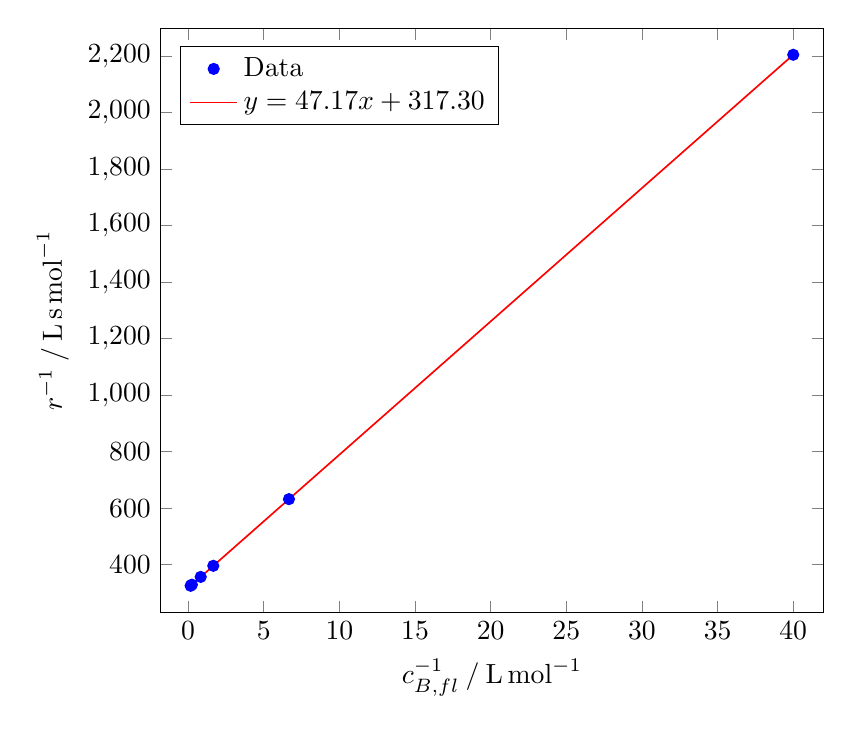
\begin{tikzpicture}
\begin{axis}[
height=9cm,
legend cell align={left},
legend pos=north west,
width=10cm,
xlabel={$ c_{B,fl}^{-1}\: / \: \si{\liter\per\mole}$},
xmin=-1.825, xmax=41.9916666666667,
ylabel={$r^{-1}\: / \: \si{\liter\second\per\mole}$},
ymin=231.206530949541, ymax=2298.21657434581,
]
\addplot [draw=blue, fill=blue, mark=*, only marks]
table{%
x  y
40 2204.26157237326
6.66666666666667 631.778456354638
1.66666666666667 395.908940943583
0.833333333333333 356.612184249629
0.25 329.109758104328
0.166666666666667 325.168003468459
};
\addlegendentry{Data}
\addplot [semithick, red]
table {%
40 2204.25883169654
6.66666666666667 631.792472889477
1.66666666666667 395.922519068417
0.833333333333333 356.61086009824
0.25 329.092698819116
0.166666666666667 325.161532922099
};
\addlegendentry{$y=47.17x+317.30$}
\end{axis}
\end{tikzpicture}

\end{center}
%%
The rate constant $k$ can be calculated by ($[m] = \si{second}$):
%%
\begin{equation}
 k = \frac{1}{m * H_A * p_A} = \pySI{k}{\liter\per\mole\second}
\end{equation}
%%
The product of the specific interface and the mass transport coefficient $a * \beta_L$ can be calculated by ($[d] = \si{\liter\second\per\mole}$):
%%
\begingroup 
\sisetup{round-precision=4}
\begin{equation}
 a * \beta_L = \frac{1}{d * H_A * p_A} = \pySI{aBetaL}{\per\second}
\end{equation}
\endgroup

%%
The concentration of the gas A in the liquid can by rearranging the mass balance $ \dot{n}_{diff} = \dot{n}_{rxn}$:
%%
\begin{align}
\begin{split}
&a * \beta_L * V_{fl} * \left( H_A * p_A - c_{A,fl}\right) = k * V_{fl} * c_{A,fl} * c_{B,fl}\\
&\Longrightarrow c_{A,fl} = \frac{a * \beta_L}{a * \beta_L + k * c_{B,fl}} * p_A * H_A
\end{split}
\end{align}
%%
The concentration of A in liquid without a further reaction can be calculated by rearranging the mass balance $\dot{n}_{diff} = 0$:
%%
\begin{align}
\begin{split}
&a * \beta_L * V_{fl} * \left( H_A * p_A - c_{A,fl}\right) = 0\\
&\Longrightarrow c_{A,fl} = H_A * p_A = \pySI{cAflwr}{\mole\per\liter}
\end{split}
\end{align}
%%
In the case of a high concentration of B $(k * c_{B,fl} \gg a * \beta_L)$ Eq. \ref{eqn8:rate} simplifies to:
%%
\begin{equation}
 r = k * a * \beta_L * H_A * p_A
\end{equation}
%%
\end{solution}



\begin{question}
During the execution of a radical polymerization at three different temperatures, the following data were collected for the respective course of the monomer concentration $c_M$. In addition the rate constants of the initiator decomposition reaction $k_z$ determined in kinetic investigations performed previously are available. The initial initiator concentrations are also given $c_{I0} = \SI{0.002}{\mole\per\liter}$.
%%
\renewcommand{\labelenumi}{\alph{enumi})}
\begin{enumerate}
\item Determine the activation energies $E_z$ and $E_{Br}$ as well the corresponding pre-exponential factors $k_{z\infty}$ and $k_{Br\infty}$.
\item Calculate for the different temperatures the polymerization time until a monomer conversion of \SI{75}{\percent} is reached.
\end{enumerate}
%%
\begin{table}[H]
\centering
\pgfplotstabletypeset[%
col sep=comma, header=false,
every head row/.style={before row={\toprule}, after row={\midrule}},
every last row/.style={after row=\bottomrule},
display columns/0/.style={column name={$\sfrac{T}{\si{\celsius}}$}, string type, column type={S[table-format=3]}},
display columns/1/.style={column name={$\sfrac{k_z}{\si{\per\second}}$}, string type, column type={S[scientific-notation=true, round-precision=3, table-format=1.3e-2]}},
]{Tables/tabkz.csv}
\end{table}
%%
The values for the time $t$ and monomer concentration $c_M$ are given in Tab. \ref{tab9:1} to \ref{tab9:3}.
\end{question}

\begin{pycode}
import pandas as pd
import numpy as np
from sklearn.linear_model import LinearRegression

R = 8.3144598 #J/(mol*K)

T = np.array([80, 100, 120]) #celsius
Tkelvin = np.array([80, 100, 120]) + 273.15 #K
kz = np.array([4.454e-13, 6.01e-12, 1.275e-11]) #s^-1
cI0 = 0.002 #mol/L
X = 0.75

t = 60*np.array([0, 50, 100, 150, 200, 300]) #s
cmT1 = 1e-3*np.array([1500, 1450, 1400, 1350, 1300, 1200]) #mol/L
cmT2 = 1e-3*np.array([1500, 1300, 1100, 950, 800, 600]) #mol/L
cmT3 = 1e-3*np.array([1500, 900, 550, 300, 200, 70]) #mol/L

df = pd.DataFrame({'t':t, 'cmT1':cmT1, 'cmT2':cmT2, 'cmT3':cmT3})

cM0 = df['cmT1'].values.reshape(-1,1)[0,0]

lm1 = LinearRegression()
lm2 = LinearRegression()
lm3 = LinearRegression()

Y1 = np.log(df['cmT1'].values.reshape(-1,1)/cM0)
X1 = np.exp(-kz[0]*df['t'].values.reshape(-1,1)/2) - 1 
lm1.fit(X1, Y1)         # perform linear regression
Ypred1 =lm1.predict(X1) # make predictions
slope1 = lm1.coef_[0,0]

Y2 = np.log(df['cmT2'].values.reshape(-1,1)/cM0)
X2 = np.exp(-kz[1]*df['t'].values.reshape(-1,1)/2) - 1 
lm2.fit(X2, Y2)         # perform linear regression
Ypred2 = lm2.predict(X2) # make predictions
slope2 = lm1.coef_[0,0]

Y3 = np.log(df['cmT3'].values.reshape(-1,1)/cM0)
X3 = np.exp(-kz[2]*df['t'].values.reshape(-1,1)/2) - 1 
lm3.fit(X3, Y3)         # perform linear regression
Ypred3 = lm3.predict(X3) # make predictions
slope3 = lm1.coef_[0,0]

kBr1 = slope1*kz[0]/(2*np.sqrt(cI0))
kBr2 = slope2*kz[1]/(2*np.sqrt(cI0))
kBr3 = slope3*kz[2]/(2*np.sqrt(cI0))
kBr = np.array([kBr1, kBr2, kBr3])

Ebr = R * np.log(kBr[0]/kBr[1]) * Tkelvin[0] * Tkelvin[1]/(Tkelvin[0] - Tkelvin[1])
Ez = R * np.log(kz[0]/kz[1]) * Tkelvin[0] * Tkelvin[1]/(Tkelvin[0] - Tkelvin[1])

kBrInf = kBr[0] * np.exp(Ebr / (R * Tkelvin[0]))
kzInf = kz[0] * np.exp(Ez / (R * Tkelvin[0]))

PolyTime = -2/kz * np.log(np.log(1-X) * kz / (2 * kBr * np.sqrt(cI0)) + 1)

exportDf1 = pd.DataFrame({'t': t, 'cmT1': cmT1, 'logCm': Y1.reshape(-1), 'expKz': X1.reshape(-1)})
pd.DataFrame(exportDf1).to_csv("Tables/tab1.csv", index=False, header=False)

exportDf2 = pd.DataFrame({'t': t, 'cmT2': cmT2, 'logCm': Y2.reshape(-1), 'expKz': X2.reshape(-1)})
pd.DataFrame(exportDf2).to_csv("Tables/tab2.csv", index=False, header=False)

exportDf3 = pd.DataFrame({'t': t, 'cmT3': cmT3, 'logCm': Y3.reshape(-1), 'expKz': X3.reshape(-1)})
pd.DataFrame(exportDf3).to_csv("Tables/tab3.csv", index=False, header=False)

exportDfKz = pd.DataFrame({'T': T, 'kz': kz})
pd.DataFrame(exportDfKz).to_csv("Tables/tabkz.csv", index=False, header=False)

exportDfKBr = pd.DataFrame({'T': T, 'kBr': kBr})
pd.DataFrame(exportDfKBr).to_csv("Tables/tabkBr.csv", index=False, header=False)

exportPolyTime = pd.DataFrame({'T': T, 'PolyTime': PolyTime})
pd.DataFrame(exportPolyTime).to_csv("Tables/polytime.csv", index=False, header=False)
\end{pycode}

\begin{solution}
The logarithmic ratio of the monomer concentration to the initial concentration can be calculated by:
%
\begin{equation}\label{eqn9:logratio}
\ln \left( \frac{c_M}{c_{M0}} \right) = \underbrace{\frac{2 * k_{Br} * \sqrt{c_{I0}}}{k_z}}_{\text{slope } m}  * \left[ \exp\left(\frac{-k_z * t}{2} \right) - 1 \right]
\end{equation}
%%
The slope can be determined by linear regression $\ln \left( \frac{c_M}{c_{M0}} \right) = f\left(\exp\left(\frac{-k_z * t}{2} \right) - 1\right)$. The gross rate constant can be calculated by:
%%
\begin{equation}\label{eqn9:kbr}
 k_{Br} = \frac{m * k_z}{2 * \sqrt{c_{I0}}}
\end{equation}
%%
Tab. \ref{tab9:1} to \ref{tab9:3} contain the results of the calculation of the slope and the logarithmic ratio
\begin{table}[H]
\caption{At \SI{80}{\celsius}}
\label{tab9:1}
\centering
\pgfplotstabletypeset[%
col sep=comma, header=false,
every head row/.style={before row={\toprule}, after row={\midrule}},
every last row/.style={after row=\bottomrule},
display columns/0/.style={column name={$\sfrac{t}{\si{\second}}$}, string type, column type={S[table-format=5]}},
display columns/1/.style={column name={$\sfrac{c_M}{\si{\mole\per\liter}}$}, string type, column type={S[round-precision=2, table-format=1.2]}},
display columns/2/.style={column name={${\ln\left(\frac{c_M}{c_{M0}}\right)}$}, string type, column type={S[scientific-notation=true, round-precision=2, table-format=-1.2e-1]}},
display columns/3/.style={column name={${\exp\left(\frac{-k_z * t}{2}\right) - 1}$}, string type, column type={S[scientific-notation=true, round-precision=2, table-format=-1.2e-2]}},
]{Tables/tab1.csv}
\end{table}
%%
\begin{table}[H]
\centering
\caption{At \SI{100}{\celsius}}
\label{tab9:2}
\pgfplotstabletypeset[%
col sep=comma, header=false,
every head row/.style={before row={\toprule}, after row={\midrule}},
every last row/.style={after row=\bottomrule},
display columns/0/.style={column name={$\sfrac{t}{\si{\second}}$}, string type, column type={S[table-format=5]}},
display columns/1/.style={column name={$\sfrac{c_M}{\si{\mole\per\liter}}$}, string type, column type={S[round-precision=2, table-format=1.2]}},
display columns/2/.style={column name={${\ln\left(\frac{c_M}{c_{M0}}\right)}$}, string type, column type={S[scientific-notation=true, round-precision=2, table-format=-1.2e-1]}},
display columns/3/.style={column name={${\exp\left(\frac{-k_z * t}{2}\right) - 1}$}, string type, column type={S[scientific-notation=true, round-precision=2, table-format=-1.2e-2]}},
]{Tables/tab2.csv}
\end{table}
%%
\begin{table}[H]
\centering
\caption{At \SI{120}{\celsius}}
\label{tab9:3}
\pgfplotstabletypeset[%
col sep=comma, header=false,
every head row/.style={before row={\toprule}, after row={\midrule}},
every last row/.style={after row=\bottomrule},
display columns/0/.style={column name={$\sfrac{t}{\si{\second}}$}, string type, column type={S[table-format=5]}},
display columns/1/.style={column name={$\sfrac{c_M}{\si{\mole\per\liter}}$}, string type, column type={S[round-precision=2, table-format=1.2]}},
display columns/2/.style={column name={${\ln\left(\frac{c_M}{c_{M0}}\right)}$}, string type, column type={S[round-precision=2, table-format=-1.2]}},
display columns/3/.style={column name={${\exp\left(\frac{-k_z * t}{2}\right)-1}$}, string type, column type={S[scientific-notation=true, round-precision=2, table-format=-1.2e-2]}},
]{Tables/tab3.csv}
\end{table}
%%
Determined regression lines:
%%
\begin{center}
 % This file was created by tikzplotlib v0.9.8.
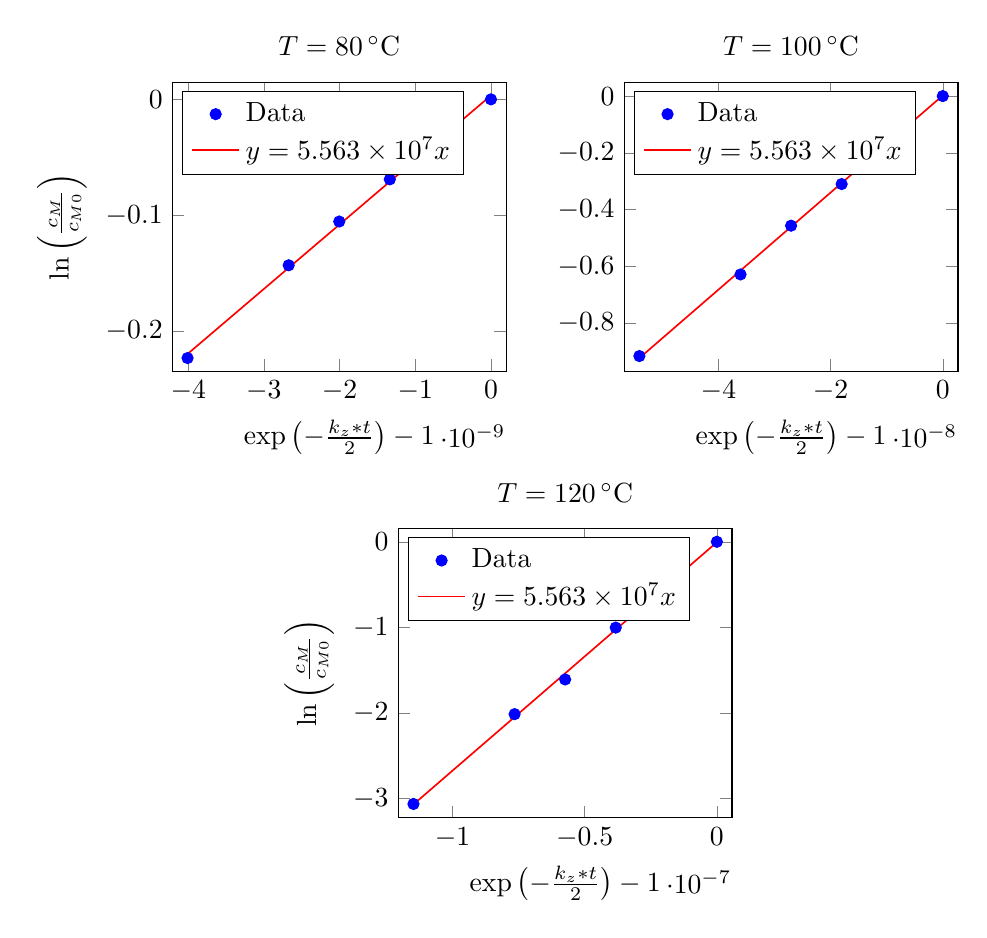
\begin{tikzpicture}


\begin{groupplot}[group style={group size=2 by 2, horizontal sep=1.5cm}, ylabel = {$\ln\left(\frac{c_M}{c_{M0}}\right)$},  xlabel = {$\exp\left(-\frac{k_z * t}{2}\right) - 1$}, height=5.25cm, width=0.48\textwidth, yticklabel style={/pgf/number format/fixed}, legend pos=north west, legend cell align={left}]
\nextgroupplot[
title = {$T = \SI{80}{\celsius}$},
xmin=-4.20903000786232e-09, xmax=2.00430000374396e-10,
ymin=-0.2344688647448, ymax=0.0146880307281916
]
\addplot [draw=blue, fill=blue, mark=*, only marks]
table{%
x  y
0 0
-6.68100019751705e-10 -0.0339015516756813
-1.33620003950341e-09 -0.0689928714869513
-2.00429994823281e-09 -0.105360515657826
-2.67239996798452e-09 -0.143100843640673
-4.00860000748793e-09 -0.22314355131421
};
\addlegendentry{Data}

\addplot [semithick, red]
table {%
0 0.0033627172976011
-6.68100019751705e-10 -0.0338045112080159
-1.33620003950341e-09 -0.0709717397136329
-2.00429994823281e-09 -0.108138962042942
-2.67239996798452e-09 -0.145306190548559
-4.00860000748793e-09 -0.219640647559793
};

\addlegendentry{$y=\num{5.563e+07}x$}

\nextgroupplot[
title = {$T = \SI{100}{\celsius}$},
xmin=-5.67944985208069e-08, xmax=2.70449992956223e-09,
ymin=-0.969634736429352, ymax=0.0484893992726729,
ylabel = {}
]
\addplot [draw=blue, fill=blue, mark=*, only marks]
table{%
x  y
0 0
-9.01499996874833e-09 -0.143100843640673
-1.80299998264744e-08 -0.310154928303839
-2.70449996842004e-08 -0.456758402495715
-3.60599993198818e-08 -0.628608659422374
-5.40899985912446e-08 -0.916290731874155
};
\addlegendentry{Data}

\addplot [semithick, red]
table {%
0 0.00221102946803542
-9.01499996874833e-09 -0.152050206697004
-1.80299998264744e-08 -0.306311440962271
-2.70449996842004e-08 -0.460572675227539
-3.60599993198818e-08 -0.614833905693264
-5.40899985912446e-08 -0.923356366624715
};
\addlegendentry{$y=\num{5.563e+07}x$}

\nextgroupplot[
title = {$T = \SI{120}{\celsius}$},
xmin=-1.20487493066035e-07, xmax=5.73749966981119e-09,
ymin=-3.22333734647094, ymax=0.153492254593854,
at = { ($ ( $ (group c1r1.south west) + (0,-4cm)$ )!0.5!(group c2r1.south east) $ ) }
]
\addplot [draw=blue, fill=blue, mark=*, only marks]
table{%
x  y
0 0
-1.91249998060528e-08 -0.510825623765991
-3.82499992790386e-08 -1.00330210886378
-5.73749983079352e-08 -1.6094379124341
-7.64999971147873e-08 -2.01490302054226
-1.14749993396224e-07 -3.06472514504094
};
\addlegendentry{Data}

\addplot [semithick, red]
table {%
0 -0.00508202551092984
-1.91249998060528e-08 -0.515875894121115
-3.82499992790386e-08 -1.02666975383569
-5.73749983079352e-08 -1.53746360168945
-7.64999971147873e-08 -2.04825744361281
-1.14749993396224e-07 -3.06984509187708
};
\addlegendentry{$y=\num{5.563e+07}x$}
\end{groupplot}

\end{tikzpicture}

\end{center}
%%
The gross rate constants from Eq. \ref{eqn9:kbr}:
%%
\begin{table}[H]
\centering
\caption{Gross reaction constants.}
\pgfplotstabletypeset[%
col sep=comma, header=false,
every head row/.style={before row={\toprule}, after row={\midrule}},
every last row/.style={after row=\bottomrule},
display columns/0/.style={column name={$\sfrac{T}{\si{\celsius}}$}, string type, column type={S[table-format=3]}},
display columns/1/.style={column name={$\sfrac{k_{Br}}{\si{\liter\tothe{1\per 2}\per\mole\tothe{1\per 2}\per\second}}$}, string type, column type={S[scientific-notation=true, round-precision=3, table-format=1.3e-2]}},
]{Tables/tabkBr.csv}
\end{table}
%%
The activation energy for the gross reaction reaction can be calculated by (temperature in kelvin):
%%
\begin{equation}
 E_{Br} = R * \ln\left[\frac{k_{Br}(T_1)}{k_{Br}(T_2)}\right] * \frac{T_1 * T_2}{T_1 - T_2} = \pySI{1e-3 * Ebr}{\kilo\joule}
\end{equation}
%%
The pre-exponential factor for the gross reaction can be calculated by:
%%
\begin{equation}
 k_{Br\infty} = k_{Br}(T_1) * \exp\left(\frac{E_{Br}}{R * T_1}\right) = \pySI{kBrInf}{\liter \pow{1\per 2} \per \mole \pow{1\per 2} \per \second}
\end{equation}
%%
The activation energy for the initiator decomposition reaction can be calculated by:
%%
\begin{equation}
 E_{z} = R * \ln\left[\frac{k_{z}(T_1)}{k_{z}(T_2)}\right] * \frac{T_1 * T_2}{T_1 - T_2} = \pySI{1e-3 * Ez}{\kilo\joule}
\end{equation}
%%
The pre-exponential factor for the initiator decomposition reaction  can be calculated by:
%%
\begin{equation}
 k_{z\infty} = k_{z}(T_1) * \exp\left(\frac{E_{z}}{R * T_1}\right) = \pySIsci{kzInf}{\liter \pow{1\per 2} \per \mole \pow{1\per 2} \per \second}
\end{equation}
%%
The conversion in constant reaction volume is defined by:
%
\begin{equation}
X = \frac{c_{M0} - c_M}{c_{M0}} \Longrightarrow \frac{c_M}{c_{M0}} = 1 - X
\end{equation}
%
Thus the polymerization time $t_p$ for a monomer conversion of \SI{75}{\percent} can be calculated by rearranging Eq. \ref{eqn9:logratio}:
%
\begin{align}
\begin{split}
&\ln \left( 1 - X \right) = \frac{2 * k_{Br} * \sqrt{c_{I0}}}{k_z} * \left[ \exp\left(\frac{-k_z * t_p}{2} \right) - 1 \right]\\
&\Longrightarrow t_p = -\frac{2}{k_z} * \ln \left[ \frac{\ln (1 - X) * k_z}{2 * k_{Br} * \sqrt{c_{I0}}} + 1 \right]
\end{split} 
\end{align}
%%
\begin{table}[H]
\centering
\caption{Polymerization times}
\pgfplotstabletypeset[%
col sep=comma, header=false,
every head row/.style={before row={\toprule}, after row={\midrule}},
every last row/.style={after row=\bottomrule},
display columns/0/.style={column name={$\sfrac{T}{\si{\celsius}}$}, string type, column type={S[table-format=3]}},
display columns/1/.style={column name={$\sfrac{t_p}{\si{\second}}$}, string type, column type={S[scientific-notation=true, round-precision=3, table-format=1.3e1]}},
]{Tables/polytime.csv}
\end{table}
\end{solution}





\begin{question}
What is meant by stationarity in a reactor system? How does this affect the mass and heat balance?
\end{question}

\begin{solution}
A \textbf{stationary process} describes the movement of matter or energy in which the state variables of the considered system do not change in the course of time.
%%
\begin{itemize}
 \item In terms of the \textbf{mass balance}, an intermediate product of a reaction chain has a constant concentration over time during the process.
 \item With regard to the \textbf{heat balance}, the continuous heat transport is stationary if the temperature at any point in the system is constant in time.
\end{itemize}
%%
This implies mathematically for the mass balance:
%%
\begin{equation}
 \frac{\mathrm{d}c_A}{\mathrm{d}t} = - \nabla * \vec{j} + \nu_A * r \overset{!}{=} 0
\end{equation}
%%
And for the heat balance:
%%
\begin{equation}
 \frac{\mathrm{d}(\rho * c_p * T)}{\mathrm{d}t} =  - \nabla * \vec{\dot{q}} + (-\Delta H)* r \overset{!}{=} 0 
\end{equation}
%%
\end{solution}


\begin{question}
Name an example of how you can reduce mass transfer limitations in a heterogeneously catalyzed reaction in the case of:
\renewcommand{\labelenumi}{(\alph{enumi})}
\begin{enumerate}
\item pore diffusion
\item film diffusion
\end{enumerate}
\end{question}

\begin{solution}
To reduce \textbf{pore diffusion}, the particle size of the catalyst can be reduced. 

To reduce \textbf{film diffusion}, the flow velocity of the fluid can be increased.

\end{solution}


\begin{question}
Radical polymerization is a system of consecutive reactions. Intermediate products are radicals.

\renewcommand{\labelenumi}{(\alph{enumi})}
\begin{enumerate}
 \item Explain the Bodenstein quasi-staionarity principle in context with radical polymerization.
 \item What is the degree of polymerization $P_n$. What measures are necessary in the process of radical polymerization to achieve the highest possible degree of polymerization $P_n$. Neglect the gel effect.
 \item What is the meaning of the radical efficiency factor?
\end{enumerate}
\end{question}

\begin{solution}
\textbf{Bodenstein's quasi-stationary principle} states that if an intermediate product (B) is formed slowly with rate constant $k_1$ and the final product (C) is formed quickly with rate constant $k_2$, it can be assumed that the concentration of the intermediate product does not change.

\begin{equation}
 \ch{A ->[ $k_1$ ] B ->[ $k_2$ ] C} \qquad \text{with } k_2 \gg k_1 
\end{equation}
%%
The \textbf{degree of polymerization} is the ratio of the number average of the molar mass of the macro molecule $M_n$ and the molar mass of the basic building block $M_m$ (monomer).
%%
\begin{equation}
 P_n = \frac{M_n}{M_m}
\end{equation}
%%
In case of a \textbf{radical polymerization} the degree of polymerization is proportional to the ratio of the rate of the propagation and the rate of the termination.
%%
\begin{equation}
 P_n \propto \frac{k_w}{k_a}
\end{equation}
%
A high degree of polymerization requires $k_w \gg k_a$.

The \textbf{radical efficiency factor} $f$ describes the effective radical concentration. The efficiency is ideal 1 but can be decreased due to recombination of the radical inside a solvent cage or before initiating a chain, or due to side reactions. 
\end{solution}


\begin{question}
What do you understand by the term catalysis? Name three different metal catalyst and the reaction catalyzed with them.

\end{question}

\begin{solution}
\textbf{Catalysis} means the lowering of the activation energy $E_a$. It is the process of increasing the rate of a chemical reaction by adding a catalyst, which is not consumed in the course of the reaction.
\vspace{-2.5cm}
\begin{center}
 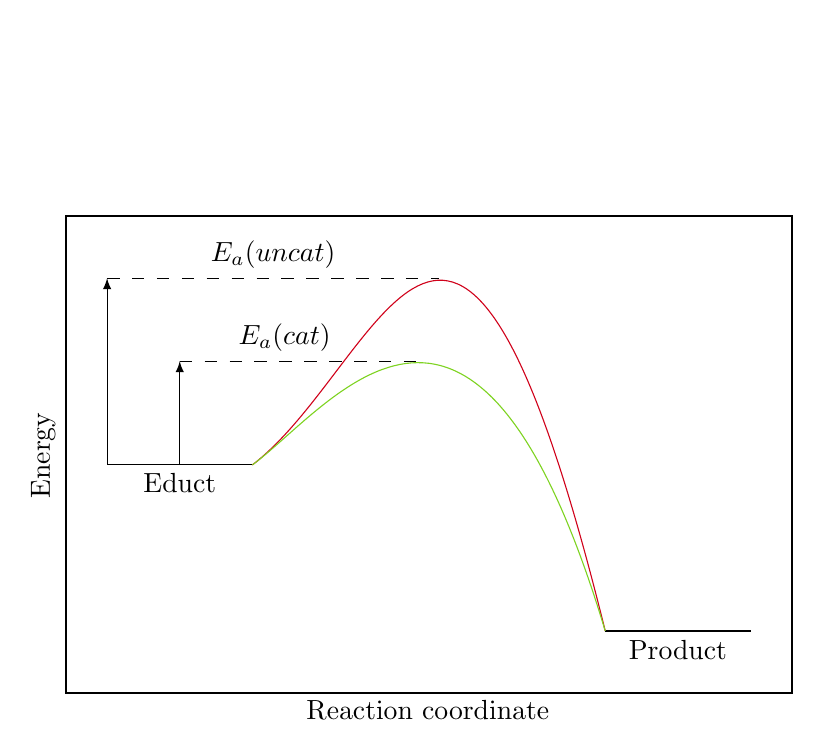
\begin{tikzpicture}[x=0.75pt,y=0.75pt,yscale=-1,xscale=1]
%\path (0,557); %set diagram left start at 0, and has height of 557
%Straight Lines [id:da8963302898593869] 
\draw    (110,130) -- (180,130) ;
%Curve Lines [id:da25528306667553147] 
\draw [color={rgb, 255:red, 208; green, 2; blue, 27 }  ,draw opacity=1 ]   (180,130) .. controls (243.78,80.98) and (278.25,-80.4) .. (350,210) ;
%Straight Lines [id:da9286679635565723] 
\draw    (350,210) -- (420,210) ;
%Curve Lines [id:da5920006668723389] 
\draw [color={rgb, 255:red, 126; green, 211; blue, 33 }  ,draw opacity=1 ]   (180,130) .. controls (220,100) and (287.55,2.25) .. (350,210) ;
%Shape: Rectangle [id:dp9170110896395716] 
\draw  [line width=0.75]  (90,10) -- (440,10) -- (440,240) -- (90,240) -- cycle ;
%Straight Lines [id:da29019500832361755] 
\draw  [dash pattern={on 4.5pt off 4.5pt}]  (110,40) -- (270,40) ;
%Straight Lines [id:da3043530571809191] 
\draw  [dash pattern={on 4.5pt off 4.5pt}]  (145,80) -- (260,80) ;
%Straight Lines [id:da6765322257918037] 
\draw [latex-]   (145,80) -- (145,130) ;
%Straight Lines [id:da6158891760080316] 
\draw [latex-]   (110,40) -- (110,130) ;

% Text Node
\draw (264.5,242) node [anchor=north] [inner sep=0.75pt]   [align=left] {Reaction coordinate};
% Text Node
\draw (72,125.5) node [anchor=north] [inner sep=0.75pt]  [rotate=-270] [align=left] {Energy};
% Text Node
\draw (195.5,76.6) node [anchor=south] [inner sep=0.75pt]    {$E_{a}( cat)$};
% Text Node
\draw (190,36.6) node [anchor=south] [inner sep=0.75pt]    {$E_{a}( uncat)$};
% Text Node
\draw (385,213) node [anchor=north] [inner sep=0.75pt]   [align=left] {Product};
% Text Node
\draw (145,133) node [anchor=north] [inner sep=0.75pt]   [align=left] {Educt};
\end{tikzpicture}

\end{center}
%%
The synthesis of methane:
%%
\begin{equation}
 \ch{CO + 3 H2 ->[Ni] CH4 + H2O}
\end{equation}
%%
The synthesis of methanol:
%%
\begin{equation}
 \ch{CO + 2 H2 ->[Zn,\;Cu-oxide] CH3OH}
\end{equation}
%%
Fischer-Tropsch synthesis:
%%
\begin{equation}
 \ch{$n$ CO + $(2n+1)$ H2 ->[Fe] C_{$n$}H_{$2n+2$} + $n$ H2O}
\end{equation}
\end{solution}

\begin{question}
A heterogeneously catalysed reaction of two gaseous reactants (\ch{A + B}) to the product C shows \textbf{Eley-Rideal} kinetics. In an experiment, the partial pressure of component B is kept constant, while that of component A is steadily increased. Describe the course of the reaction rate and explain it using a suitable formula.  For this purpose, assign the areas of the curve exactly to the explained cases (in the diagram)! 

\end{question}
\begin{solution}
The Eley-Rideal model states that one reactant is chemisorpt on the surface of the catalyst.
%%
\begin{equation*}
\ch{A_{ch} + B_{g} -> C}
\end{equation*}
%%
The reaction rate can be described by:
%%
\begin{equation}
r = k * \Theta_A * p_B
\end{equation}
%%
The coverage $\Theta$ can be calculated by:
%%
\begin{equation}
\Theta_A = \frac{K_A * p_A}{1 + K_A * p_A}
\end{equation}
%%
Thus the reaction rate can be rearranged to:
%%
\begin{equation}\label{eqn14:rate}
r = k * \frac{K_A * p_A * p_B}{1 + K_A * p_A}
\end{equation}
%%
In the case of a low partial pressure of A $(K_A * p_A \ll 1)$, Eq. \ref{eqn14:rate} can be simplified to:
%%
\begin{equation}
r = k * K_A *  p_A * p_B
\end{equation}
%%
The reaction is 2nd order and the rate behaves 1st order in $p_A$. 

In the case of a high partial pressure of A $(K_A * p_A \gg 1)$, Eq. \ref{eqn14:rate} can be simplified to:
%%
\begin{equation}
r = k * p_B 
\end{equation}
%%
The reaction is 1st order and the rate behaves zero order in $p_A$. 
%%
\begin{center}
% This file was created by tikzplotlib v0.9.8.
\begin{tikzpicture}

\definecolor{color0}{rgb}{0.12156862745098,0.466666666666667,0.705882352941177}

\begin{axis}[
height=9cm,
width=10cm,
ylabel near ticks,
xlabel near ticks,
xtick=\empty,
ytick=\empty,
xlabel={$p_A$},
xmin=0, xmax=1.05,
ylabel={$r$},
ymin=0, ymax=1.5
]
\addplot [semithick, color0]
table {%
0 0
0.0101010101010101 0.0960760977047176
0.0202020202020202 0.182921578859269
0.0303030303030303 0.261423285081202
0.0404040404040404 0.33238285370617
0.0505050505050505 0.39652490388284
0.0606060606060606 0.454504436179757
0.0707070707070707 0.50691352126684
0.0808080808080808 0.554287345974482
0.0909090909090909 0.597109678470867
0.101010101010101 0.635817808366385
0.111111111111111 0.670807012192094
0.121212121212121 0.702434589852435
0.131313131313131 0.731023513271317
0.141414141414141 0.756865724490533
0.151515151515152 0.780225116899746
0.161616161616162 0.801340230041529
0.171717171717172 0.820426685510056
0.181818181818182 0.837679388818152
0.191919191919192 0.853274519717549
0.202020202020202 0.867371331296937
0.212121212121212 0.880113776229699
0.222222222222222 0.891631976778104
0.232323232323232 0.902043553565238
0.242424242424242 0.911454826683711
0.252525252525253 0.919961901406528
0.262626262626263 0.927651649587094
0.272727272727273 0.93460259677014
0.282828282828283 0.940885724072487
0.292929292929293 0.946565193022242
0.303030303030303 0.95169900075827
0.313131313131313 0.956339572280654
0.323232323232323 0.960534295800047
0.333333333333333 0.964326006652748
0.343434343434343 0.967753424723096
0.353535353535354 0.970851549840042
0.363636363636364 0.973652019185551
0.373737373737374 0.976183430364602
0.383838383838384 0.978471633435884
0.393939393939394 0.980539994885321
0.404040404040404 0.982409636238053
0.414141414141414 0.984099649745507
0.424242424242424 0.985627293350097
0.434343434343434 0.987008166918475
0.444444444444444 0.988256371542979
0.454545454545455 0.989384653538023
0.464646464646465 0.990404534601874
0.474747474747475 0.991326429472986
0.484848484848485 0.992159752282388
0.494949494949495 0.992913012688135
0.505050505050505 0.993593902773542
0.515151515151515 0.994209375596577
0.525252525252525 0.994765716192531
0.535353535353535 0.995268605755032
0.545454545454546 0.995723179650791
0.555555555555556 0.996134079860527
0.565656565656566 0.996505502381566
0.575757575757576 0.996841240076183
0.585858585858586 0.99714472140325
0.595959595959596 0.997419045428685
0.606060606060606 0.99766701347225
0.616161616161616 0.997891157713834
0.626262626262626 0.998093767051364
0.636363636363636 0.998276910474385
0.646464646464647 0.998442458192002
0.656565656565657 0.998592100730926
0.666666666666667 0.99872736619866
0.676767676767677 0.9988496358881
0.686868686868687 0.998960158382911
0.696969696969697 0.999060062307712
0.707070707070707 0.999150367853272
0.717171717171717 0.999231997194414
0.727272727272727 0.999305783907001
0.737373737373737 0.999372481480181
0.747474747474748 0.999432771010802
0.757575757575758 0.999487268158589
0.767676767676768 0.999536529433081
0.777777777777778 0.999581057876552
0.787878787878788 0.999621308200937
0.797979797979798 0.999657691431223
0.808080808080808 0.999690579102722
0.818181818181818 0.999720307055081
0.828282828282828 0.999747178861784
0.838383838383838 0.999771468930161
0.848484848484849 0.999793425303556
0.858585858585859 0.999813272194275
0.868686868686869 0.999831212273182
0.878787878787879 0.999847428739315
0.888888888888889 0.999862087190663
0.898989898989899 0.999875337315208
0.909090909090909 0.999887314419492
0.919191919191919 0.999898140810335
0.929292929292929 0.999907927043793
0.939393939393939 0.99991677305413
0.94949494949495 0.999924769174313
0.95959595959596 0.999931997058472
0.96969696969697 0.999938530515726
0.97979797979798 0.999944436263903
0.98989898989899 0.999949774610841
1 0.999954600070238
};
\draw (axis cs:0.08,0.2) node[
  anchor=base west,
  text=black,
  rotate=70
]{1st order};
\draw (axis cs:0.75,1.05) node[
  anchor=base west,
  text=black,
  rotate=0.0
]{zero order};
\end{axis}

\end{tikzpicture}

\end{center}
\end{solution}


\begin{question}
To determine kinetic data, the reaction rate of chemical reaction is determined
\renewcommand{\labelenumi}{(\alph{enumi})}
\begin{enumerate}
\item What is the dimension of the reaction rate?
\item What are the dimension of the rate constant?
\end{enumerate}
\end{question}

\begin{solution}
The general rate law can be formulated by:
%%
\begin{equation}
 r = \frac{1}{\nu_i} * \frac{\mathrm{d}c_i}{\mathrm{d}t} = k * c_i^n \qquad \text{with } [r] = \si{\mole\per\liter\per\second}
\end{equation}
%
\begin{table}[H]
 \centering
 \caption{Rate law and dimension of $k$}
 \begin{tabular}{l l l}
 \toprule
  Order & Rate law & $[k]$ \\
  \midrule
  0 & $r = k$               & \si{\mole\per\liter\per\second} \\
  1 & $r = k*c_A $          & \si{\liter\per\second\per\mole} \\
  2 & $r = k*c_A*c_B $      & \si{\square\liter\per\square\second\per\square\mole} \\
  3 & $r = k*c_A*c_B*c_C $  & \si{\cubic\liter\per\cubic\second\per\cubic\mole} \\
  \bottomrule
 \end{tabular}
\end{table}
%%
The rate constant of a reaction with oder $n \neq 0$ has the dimension $[k] = \si{\liter\tothe{n}\second\tothe{-n}\mole\tothe{-n}}$
\end{solution}

\end{document}
